\documentclass[11pt]{article}

\usepackage[margin=1in]{geometry}
\usepackage{amsmath,amssymb}
\usepackage{graphicx}
\usepackage{booktabs}
\usepackage{array}
\usepackage{longtable}
\usepackage{caption}
\usepackage{subcaption}
\usepackage{natbib}
\usepackage{xcolor}
\usepackage{microtype}
\usepackage{hyperref}

\hypersetup{
    colorlinks=true,
    linkcolor=blue!50!black,
    citecolor=blue!50!black,
    urlcolor=blue!50!black
}

\graphicspath{{./}{../}}
\newcommand{\StrictSessionCount}{6}
\newcommand{\StrictActiveMedianGain}{0.061}
\newcommand{\StrictEntropyMedianGain}{0.063}
\newcommand{\StrictSpeedMedianGain}{0.008}
\newcommand{\StrictActiveLagOne}{0.042}
\newcommand{\StrictActiveLagFour}{0.077}
\newcommand{\StrictEntropyLagOne}{0.038}
\newcommand{\StrictEntropyLagFour}{0.081}


\title{Controlled Organizational Memory in Spontaneous Neural Population Dynamics:\\
A Six-Session HRSM State-Space Analysis of Allen Neuropixels Data}

\author{Stephen Atalebe\\
\emph{Masaryk University, Brno, Czech Republic}}

\date{\today}

\begin{document}

\maketitle

\begin{abstract}
Spontaneous neural activity is often treated either as background variability or as an internally structured dynamical process. This study asks whether spontaneous neural population states contain a retained historical component that improves prediction of future population organization. Six strict fixed-scale Allen Brain Observatory Visual Coding Neuropixels spontaneous sessions were analyzed using a reduced homeostatic state-space model with four operational coordinates: \(H\), \(R\), \(S\), and \(M\). Each strict session used four target regions, twenty units per region, fifteen spontaneous presentations, and matched binning. For each session, population activity was binned, projected into HRSM state space, and tested using aligned lag-history predictors against shuffled-lag controls. Across the strict cohort, active-unit fraction and population-rate entropy were the strongest cross-session controlled-memory targets, with median observed-minus-shuffled gains of \StrictActiveMedianGain{} and \StrictEntropyMedianGain{}, respectively. Variance and autocorrelation residualization preserved these two targets as the leading residualized targets. Lag-ablation tests showed that both recruitment and entropy remained positive across all tested lag settings, with controlled gain increasing across a short recent-history window. Session-level heterogeneity remained, including one strict stress-test session in which mean-rate memory was not uniformly above shuffled controls. These results support a bounded conclusion: spontaneous neural population activity carries controlled organizational memory, most visible in population recruitment and entropy, without implying consciousness, awareness, or a complete theory of neural dynamics.
\end{abstract}

\noindent\textbf{Keywords:} spontaneous neural activity; Neuropixels; Allen Brain Observatory; Allen Visual Coding; population dynamics; non-Markovian memory; entropy; recruitment; HRSM; state-space analysis.

\section{Introduction}

Neural population activity is commonly represented as an instantaneous state vector. Such a representation is necessary for modeling population dynamics, but it may be incomplete. If two neural populations occupy similar current states while differing in recent history, their future organization may still diverge. The present work asks whether such reduced-state incompleteness can be detected operationally in spontaneous neural activity. The test is statistical rather than metaphysical: does aligned recent population history improve prediction of future population organization relative to a present-state baseline and relative to a shuffled-lag null?

Spontaneous neural activity is not empty baseline. Large-scale recordings have shown that spontaneous activity can be high-dimensional, structured, and related to ongoing behavior or internal state \citep{Stringer2019Spontaneous}. Work on latent neural states has emphasized that neural variability is shaped by non-stationary internal dynamics, behavioral context, and stimulus context \citep{Akella2025LatentStates}. Hidden-state analyses of spontaneous spiking activity similarly indicate that ongoing population activity can be organized into latent dynamical regimes \citep{Sederberg2024LatentDynamics}. These results motivate a narrower and directly testable question: whether retained recent history contributes to prediction of future spontaneous population organization.

The analysis uses the Allen Brain Observatory Visual Coding Neuropixels dataset, a public Allen Institute resource built from large-scale extracellular recordings in the mouse visual system and associated cortical, thalamic, hippocampal, and related structures \citep{AllenBrainObservatoryVisualCodingNeuropixels,Jun2017Neuropixels,Siegle2021VisualHierarchy}. The Allen Brain Observatory provides standardized and reusable neurophysiology datasets, and its Visual Coding resources have become a reference point for analyses of visual coding, open neurophysiology, and population dynamics \citep{DeVries2023AllenLessons,Xie2023VisualCodingAssessment}. Access conventions and metadata structure were cross-checked against the AllenSDK Visual Coding Neuropixels documentation \citep{AllenSDKVisualCodingNeuropixels}. Here, the stimulus-driven components of the dataset are not the primary focus. Instead, spontaneous intervals are used to test whether ongoing population dynamics carry controlled historical structure.

The framework used here is a reduced homeostatic state-space model, abbreviated HRSM. The four coordinates are operational proxies rather than direct physiological observables. \(H\) summarizes organized reserve-like population magnitude and recruitment, \(R\) summarizes recoverability-like low local deformation, \(S\) summarizes stability-like distributional coherence, and \(M\) summarizes retained recent population structure. The important empirical test is not the existence of an \(M\) coordinate by definition. It is whether aligned recent-history predictors improve target prediction beyond a shuffled-lag control.

The manuscript deliberately uses bounded language. The result is not presented as independent external replication, because all sessions come from the Allen Brain Observatory Visual Coding Neuropixels dataset. It is within-dataset cross-session generalization across six strict fixed-scale sessions. The result is also not presented as universal mean-rate memory. The strongest cross-session evidence concerns organizational targets, especially active-unit fraction and population-rate entropy.

\section{Data and preprocessing}

\subsection{Dataset provenance}

No new animal experiments were performed. The study reuses public Allen Brain Observatory Visual Coding Neuropixels data \citep{AllenBrainObservatoryVisualCodingNeuropixels}. The Visual Coding Neuropixels resource contains in vivo extracellular electrophysiology recordings collected with high-density Neuropixels probes, together with unit metadata, electrode metadata, stimulus/presentation tables, and session identifiers needed for reproducible extraction. The present analysis uses only spontaneous-presentation intervals. The visual-stimulus components of the dataset are retained as part of the public data context but are not modeled as stimulus responses in this manuscript.

\subsection{Strict fixed-scale session cohort}

Six Allen Visual Coding Neuropixels sessions were included in the strict fixed-scale cohort:
\[
715093703,\quad
719161530,\quad
750749662,\quad
751348571,\quad
755434585,\quad
756029989.
\]
Each strict session contributed four target regions:
\[
\mathrm{VISp},\quad \mathrm{VISl},\quad \mathrm{LGd},\quad \mathrm{CA1}.
\]
Each region contributed twenty selected units. Each session used fifteen spontaneous presentations, a 0.25 second bin size, and a maximum duration of 60 seconds per spontaneous presentation. Session 754312389 was excluded from the strict cohort and retained only as a partial-coverage diagnostic because VISl contributed fewer than twenty units. This fixed-scale design was chosen to avoid making cross-session differences depend trivially on the number of retained units per region.

\begin{table}[t]
\centering
\caption{Strict six-session extraction summary. Each strict session used four regions, twenty units per region, fifteen spontaneous presentations, and matched binning.}
\label{tab:strict-extraction}
\resizebox{\textwidth}{!}{%
\begin{tabular}{lrrrrl}
\toprule
Session & Units & Min/region & Presentations & Binned rows & Regions \\
\midrule
715093703 & 80 & 20 & 15 & 169280 & CA1,LGd,VISl,VISp \\
719161530 & 80 & 20 & 15 & 169280 & CA1,LGd,VISl,VISp \\
750749662 & 80 & 20 & 15 & 169280 & CA1,LGd,VISl,VISp \\
751348571 & 80 & 20 & 15 & 169280 & CA1,LGd,VISl,VISp \\
755434585 & 80 & 20 & 15 & 169360 & CA1,LGd,VISl,VISp \\
756029989 & 80 & 20 & 15 & 169280 & CA1,LGd,VISl,VISp \\
\bottomrule
\end{tabular}%
}

\end{table}

The analysis used direct HDF5 access to cached NWB files rather than constructing full PyNWB session objects. This was a computational choice intended to reduce memory pressure while preserving access to spike times, unit identifiers, electrode-region metadata, and spontaneous-presentation intervals. The derived tables used in this manuscript therefore represent a low-memory extraction of public Allen data rather than a new primary dataset.

\subsection{Population-state matrix}

For each session and region, binned spike counts were converted into a population-state matrix. Each row represented one time-bin population state within one spontaneous presentation. The main target variables were population mean rate, population rate standard deviation, active-unit fraction, population L2 rate norm, population-rate entropy, and population-state speed. Active-unit fraction quantifies recruitment. Population-rate entropy quantifies the distributional organization of population activity. Population-state speed measures local deformation between successive population states.

All target variables were computed inside session-region trajectories, preserving the spontaneous-presentation structure. Bins at the beginning of a trajectory were handled separately when lagged predictors were unavailable. The same binning and target definitions were used across all strict sessions.

\section{Neural HRSM state-space projection}

\subsection{Raw proxy definitions}

Each population state was first mapped into raw HRSM proxy coordinates. Let \(z(\cdot)\) denote robust median/MAD standardization, with a standard-deviation fallback when the median absolute deviation is numerically zero. For each time bin, the raw neural proxy coordinates were defined as:
\[
H_{\rm raw}
=
\frac{1}{4}
\left[
z(\bar r)
+
z(f_{\rm active})
+
z(\lVert r\rVert_2)
+
z(r_{\max})
\right],
\]
where \(\bar r\) is the population mean firing rate, \(f_{\rm active}\) is active-unit fraction, \(\lVert r\rVert_2\) is the population L2 rate norm, and \(r_{\max}\) is the maximum unit rate in the bin. This coordinate is reserve-like only in the operational sense that it summarizes the organized magnitude and recruitment of the population state.

Recoverability-like return structure was defined as low local deformation:
\[
R_{\rm raw} = -z(v_{\rm state}),
\]
where \(v_{\rm state}\) is population-state speed. A low-speed state is not automatically recovered or healthy; the term recoverability is used here only as a reduced-state proxy for low local deformation.

The raw stability coordinate combined distributional organization with low local dispersion and low local deformation:
\[
S_{\rm raw}
=
\frac{1}{4}
\left[
z(E_r)
-
z(\sigma_r)
-
z(|\Delta \bar r|)
-
z(|\Delta E_r|)
\right],
\]
where \(E_r\) is population-rate entropy, \(\sigma_r\) is the across-unit rate standard deviation, and \(\Delta\) denotes the change from the previous bin within the same presentation trajectory.

The raw retained-history coordinate summarized available lagged population structure:
\[
M_{\rm raw}
=
w_{\rm hist}
\frac{1}{4}
\left[
z(\bar r_{t-1})
+
z(f_{{\rm active},t-1})
+
z(\lVert r_{t-1}\rVert_2)
+
z(E_{r,t-1})
\right],
\]
where \(w_{\rm hist}=1\) for bins with available lag history and \(w_{\rm hist}=0.25\) for the first bin of each trajectory after median lag imputation. This coordinate is a state-space retained-history proxy; the formal memory test is performed separately using aligned lag-history prediction and shuffled-lag controls.

The raw neural potential was:
\[
\Phi_{{\rm neural,raw}}
=
\frac{H_{\rm raw}+R_{\rm raw}+S_{\rm raw}+M_{\rm raw}}{4}.
\]

\subsection{Sequential residualization and axis audit}

The final \(H\), \(R\), \(S\), and \(M\) coordinates were obtained by sequential residualization in the order \(H \rightarrow R \rightarrow S \rightarrow M\). Thus \(H\) was retained as \(H_{\rm raw}\), \(R\) was residualized against \(H\), \(S\) was residualized against \(H\) and \(R\), and \(M\) was residualized against \(H\), \(R\), and \(S\). The final neural potential was:
\[
\Phi_{\rm neural}
=
\frac{H+R+S+M}{4}.
\]

The near-zero post-residualization correlations should not be interpreted as an independent biological discovery. They are a numerical verification that the residualization step worked. The biologically relevant audit is the raw pre-residualization correlation structure, which is reported alongside the post-residualization matrix.

\begin{table}[t]
\centering
\caption{Raw and orthogonalized HRSM axis audit. Raw correlations summarize pre-residualization axis overlap. Orthogonalized correlations verify numerical residualization and are not treated as independent biological evidence.}
\label{tab:axis-audit}
\resizebox{\textwidth}{!}{%
\begin{tabular}{lrrrr}
\toprule
Session & Max raw $|r|$ & Mean raw $|r|$ & Max orth. $|r|$ & Mean orth. $|r|$ \\
\midrule
715093703.0 & 0.796 & 0.343 & 3.98e-15 & 1.38e-15 \\
719161530.0 & 0.878 & 0.333 & 4.17e-15 & 1.55e-15 \\
750749662.0 & 0.818 & 0.361 & 6.16e-15 & 2.46e-15 \\
751348571.0 & 0.821 & 0.347 & 6.65e-15 & 1.73e-15 \\
755434585.0 & 0.683 & 0.328 & 1.85e-15 & 5.29e-16 \\
756029989.0 & 0.787 & 0.327 & 5.09e-15 & 1.69e-15 \\
\bottomrule
\end{tabular}%
}

\end{table}

\begin{figure}[t]
\centering
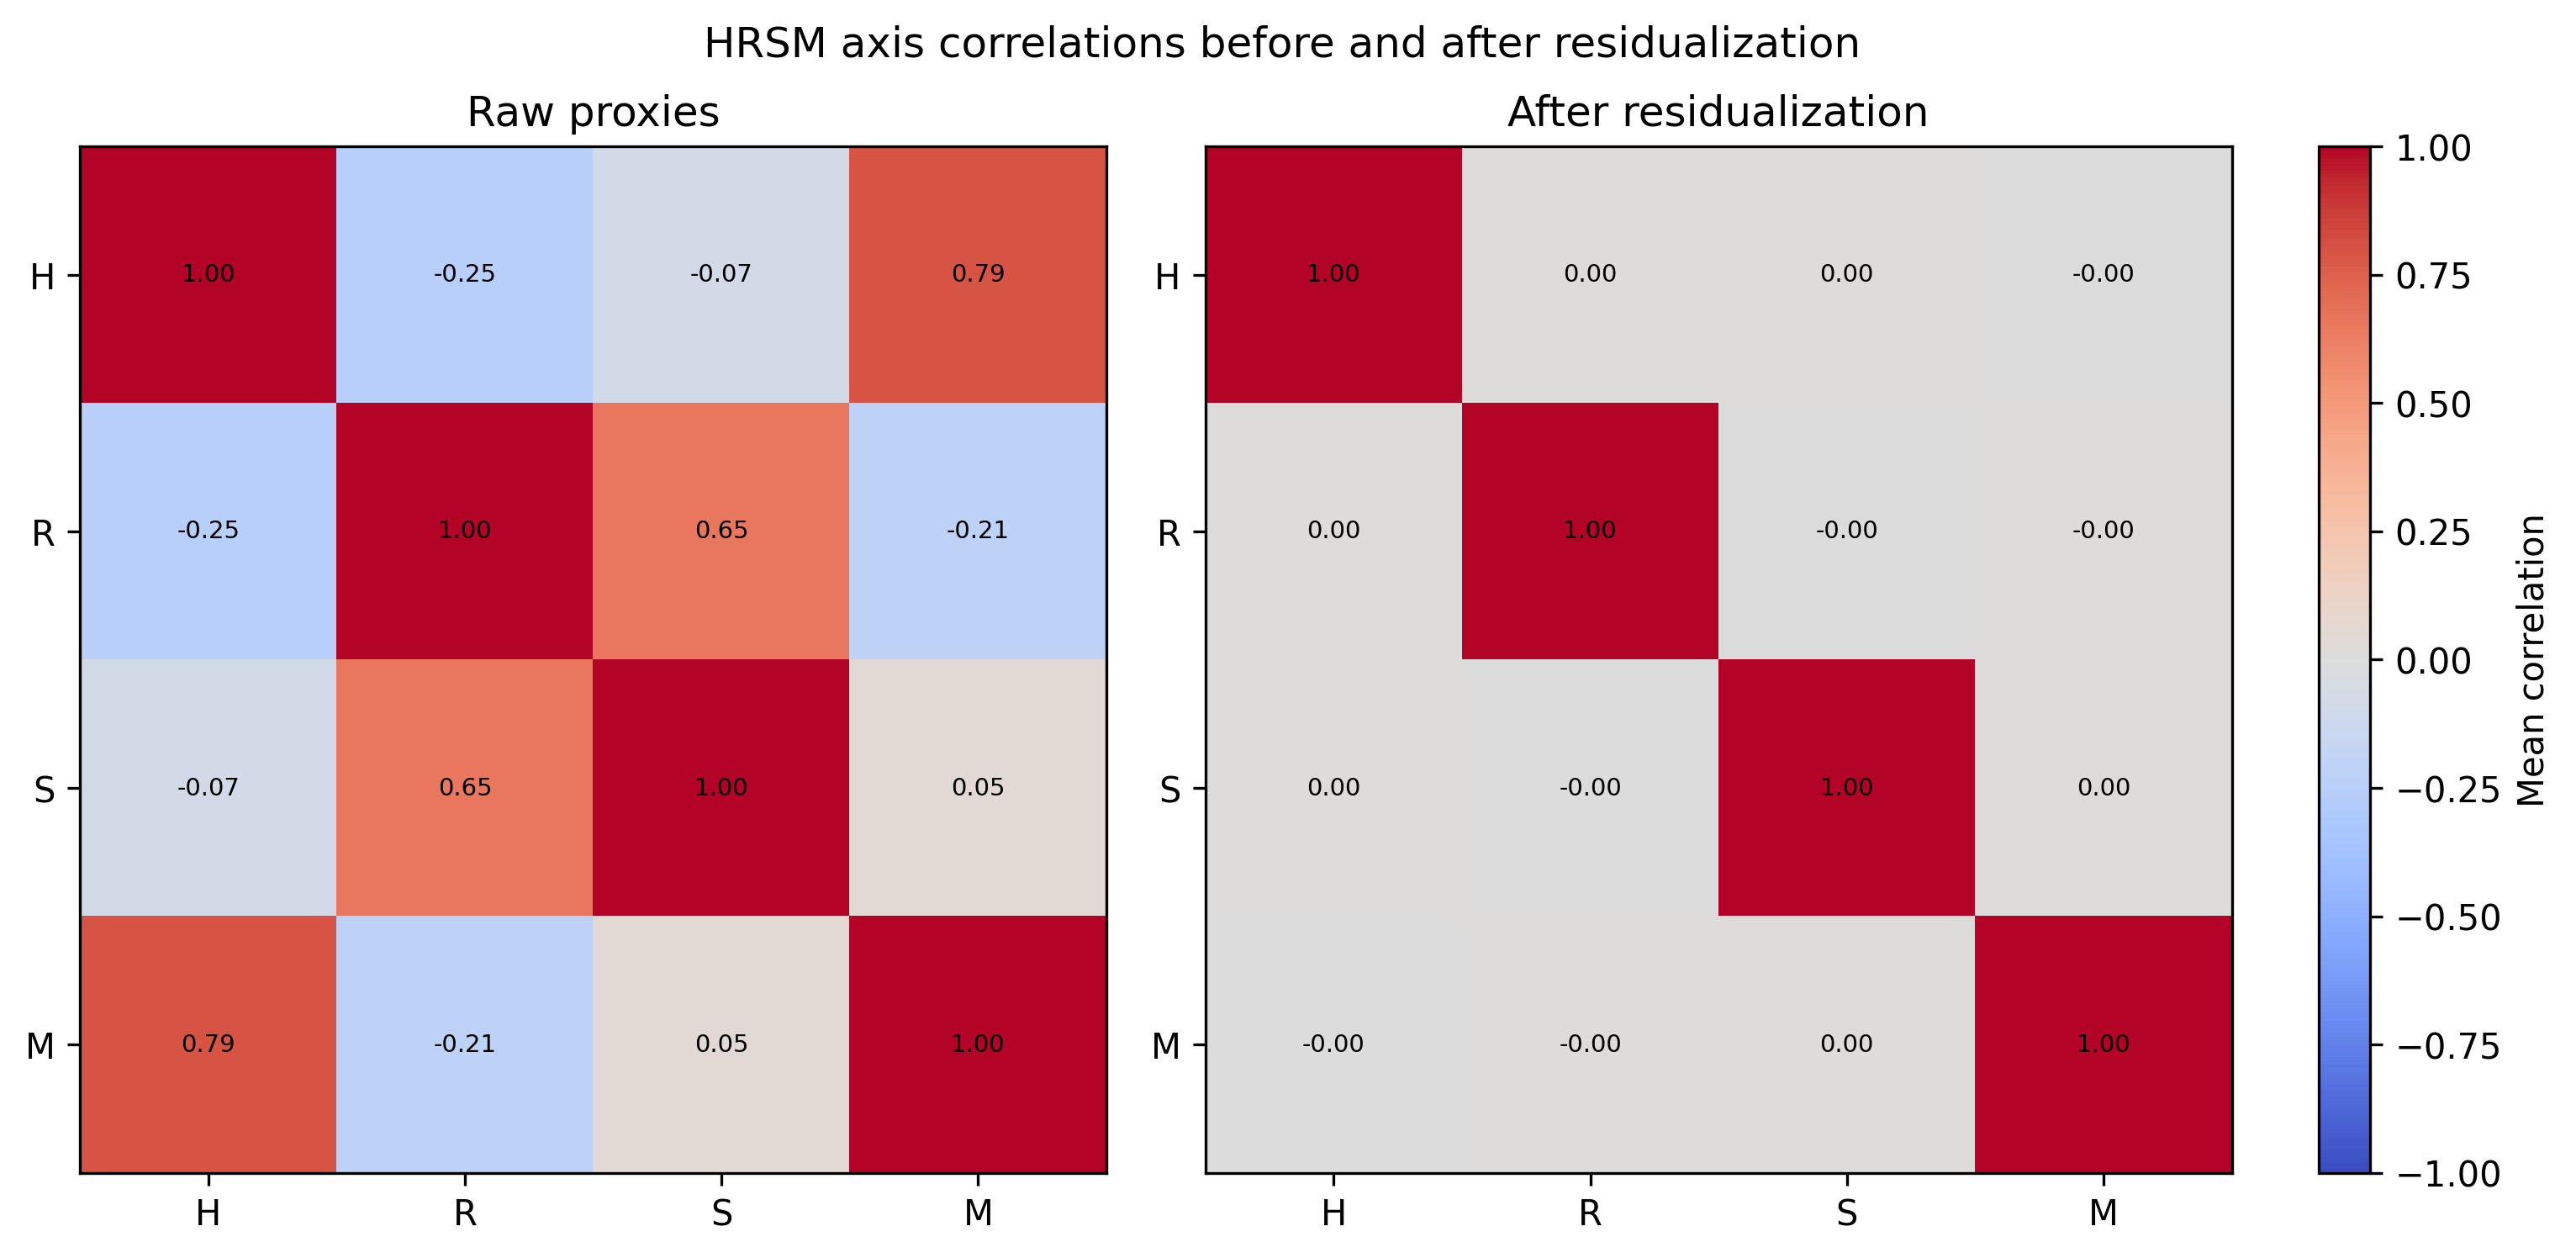
\includegraphics[width=0.88\linewidth]{results/figures/manuscript/allen_spontaneous_strict_v2/strict_v2_raw_vs_orthogonal_axis_correlations.png}
\caption{HRSM axis correlations before and after residualization. Raw proxy axes show substantial overlap, whereas post-residualization correlations are near numerical zero. The latter confirms the computation and is not interpreted as independent biological evidence.}
\label{fig:raw-orth-axis-corr}
\end{figure}

\section{Memory model and shuffled-lag control}

For each target \(y_t\), a baseline model was compared against a memory model containing aligned lag-history features. The main model used lags \((1,2)\). Additional ablation models used lag sets \((1)\), \((2)\), \((1,2)\), \((1,2,3)\), and \((1,2,3,4)\). Ridge regression was used in the main audits.

Raw memory gain was defined as:
\[
\Delta R^2_{\rm raw}
=
R^2_{\rm memory}
-
R^2_{\rm baseline}.
\]
To distinguish aligned historical contribution from distributional lag-feature effects, shuffled-lag controls were generated. The lag-feature rows were temporally shuffled relative to the target so that lag-feature distributions were retained while chronological alignment with the target was disrupted. Controlled memory gain was defined as:
\[
\Delta R^2_{\rm controlled}
=
\Delta R^2_{\rm observed}
-
\mathbb{E}
\left[
\Delta R^2_{\rm shuffled}
\right].
\]
This statistic is the primary memory quantity in the manuscript.

The shuffled-lag baseline is stricter than a simple uncontrolled lagged-model comparison because it preserves the marginal distribution of each lag component while disrupting its chronological alignment with the target. This control reduces the risk that apparent memory gain is driven only by target dispersion, static variance, or generic model inflation. A positive \(\Delta R^2_{\rm controlled}\) therefore indicates that the aligned recent past carries predictive structure beyond a temporally disrupted lag history.

\section{Results}

\subsection{Session-level synthesis shows memory with retained heterogeneity}

The strict cohort produced a cross-session synthesis with six fixed-scale spontaneous sessions. The session-level summary is shown in Figure~\ref{fig:session-overview} and Table~\ref{tab:strict-session-summary}. Five of six sessions had LGd as the highest-\(\Phi_{\rm neural}\) region, while session 750749662 had CA1 as the highest-\(\Phi_{\rm neural}\) region. This prevents a universal LGd-dominance claim. Mean-rate memory was also heterogeneous: session 755434585 did not show all-region positive mean-rate controlled memory. These exceptions sharpen the interpretation: the robust result is not universal mean-rate memory, but target-level controlled organizational memory.

\begin{figure}[t]
\centering
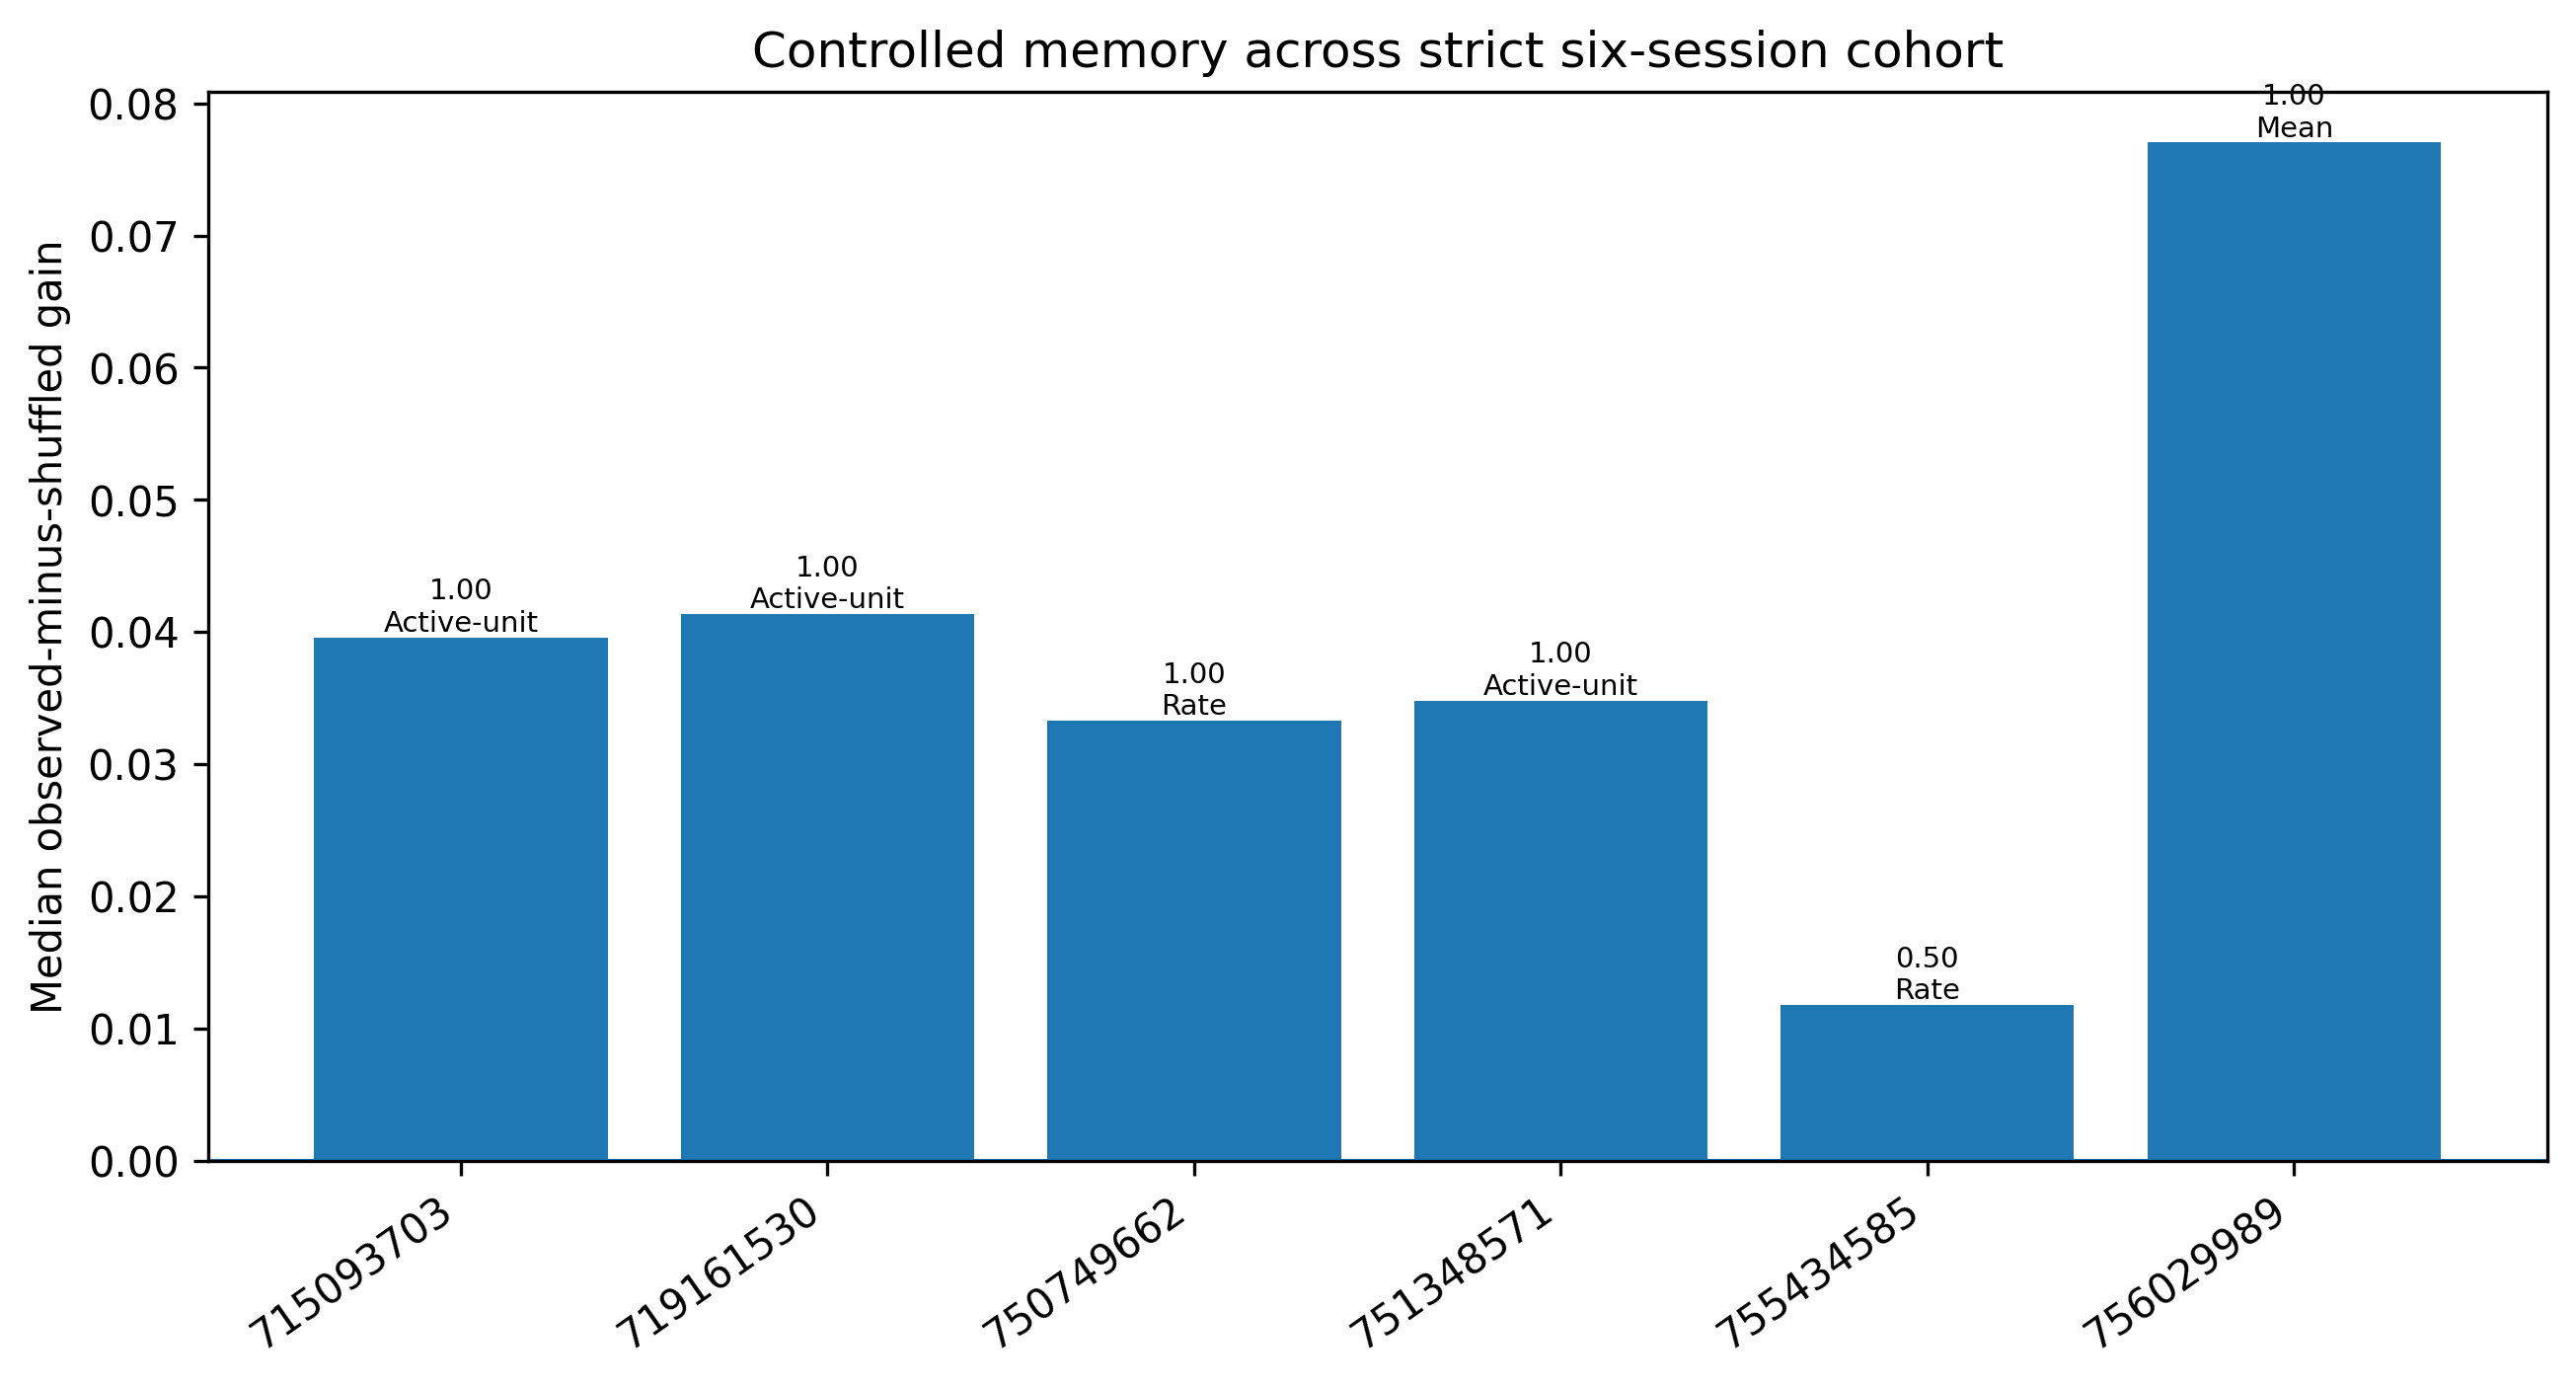
\includegraphics[width=0.88\linewidth]{results/figures/manuscript/allen_spontaneous_strict_v2/strict_v2_session_controlled_memory_overview.png}
\caption{Six-session overview of controlled memory. Bars show median observed-minus-shuffled gain by session. Annotations summarize the fraction of region-level groups above shuffled controls and the session's strongest target.}
\label{fig:session-overview}
\end{figure}

\begin{table}[t]
\centering
\caption{Strict six-session HRSM and memory summary. Session-level heterogeneity is retained rather than hidden.}
\label{tab:strict-session-summary}
\resizebox{\textwidth}{!}{%
\begin{tabular}{llrrrl}
\toprule
Session & Best $\Phi$ region & Best $\Phi$ & Median controlled gain & Frac. above shuffle & Top target \\
\midrule
715093703 & LGd & 0.408 & 0.040 & 1.00 & active\_unit\_fraction \\
719161530 & LGd & 0.703 & 0.041 & 1.00 & active\_unit\_fraction \\
750749662 & CA1 & 0.418 & 0.033 & 1.00 & population\_rate\_entropy \\
751348571 & LGd & 0.574 & 0.035 & 1.00 & active\_unit\_fraction \\
755434585 & LGd & 0.490 & 0.012 & 0.50 & population\_rate\_entropy \\
756029989 & LGd & 0.355 & 0.077 & 1.00 & population\_mean\_rate\_hz \\
\bottomrule
\end{tabular}%
}

\end{table}

\subsection{Controlled memory is strongest for recruitment and entropy}

Across six strict sessions, active-unit fraction and population-rate entropy were the strongest cross-session controlled-memory targets. The median observed-minus-shuffled gain was \StrictActiveMedianGain{} for active-unit fraction and \StrictEntropyMedianGain{} for population-rate entropy. Population-state speed ranked last. Figure~\ref{fig:strict-target-heatmap} shows that the target-level pattern is not driven by a single session: recruitment and entropy remain among the leading targets across the strict cohort, even though the strongest individual target varies by session.

\begin{table}[t]
\centering
\caption{Strict six-session target synthesis. Active-unit fraction and population-rate entropy are the strongest cross-session controlled-memory targets.}
\label{tab:strict-target-synthesis}
\resizebox{\textwidth}{!}{%
\begin{tabular}{lrrrrrr}
\toprule
Target & $n$ & Median controlled gain & Mean controlled gain & Min frac. above shuffle & Median $p$ & Rank \\
\midrule
active\_unit\_fraction & 6 & 0.061 & 0.049 & 0.75 & 0.010 & 1 \\
population\_rate\_entropy & 6 & 0.063 & 0.055 & 1.00 & 0.010 & 2 \\
population\_mean\_rate\_hz & 6 & 0.037 & 0.042 & 0.50 & 0.010 & 3 \\
population\_l2\_rate\_norm & 6 & 0.029 & 0.037 & 0.50 & 0.010 & 4 \\
population\_std\_rate\_hz & 6 & 0.029 & 0.036 & 0.50 & 0.010 & 5 \\
population\_state\_speed & 6 & 0.008 & 0.007 & 0.25 & 0.054 & 6 \\
\bottomrule
\end{tabular}%
}

\end{table}

\begin{figure}[t]
\centering
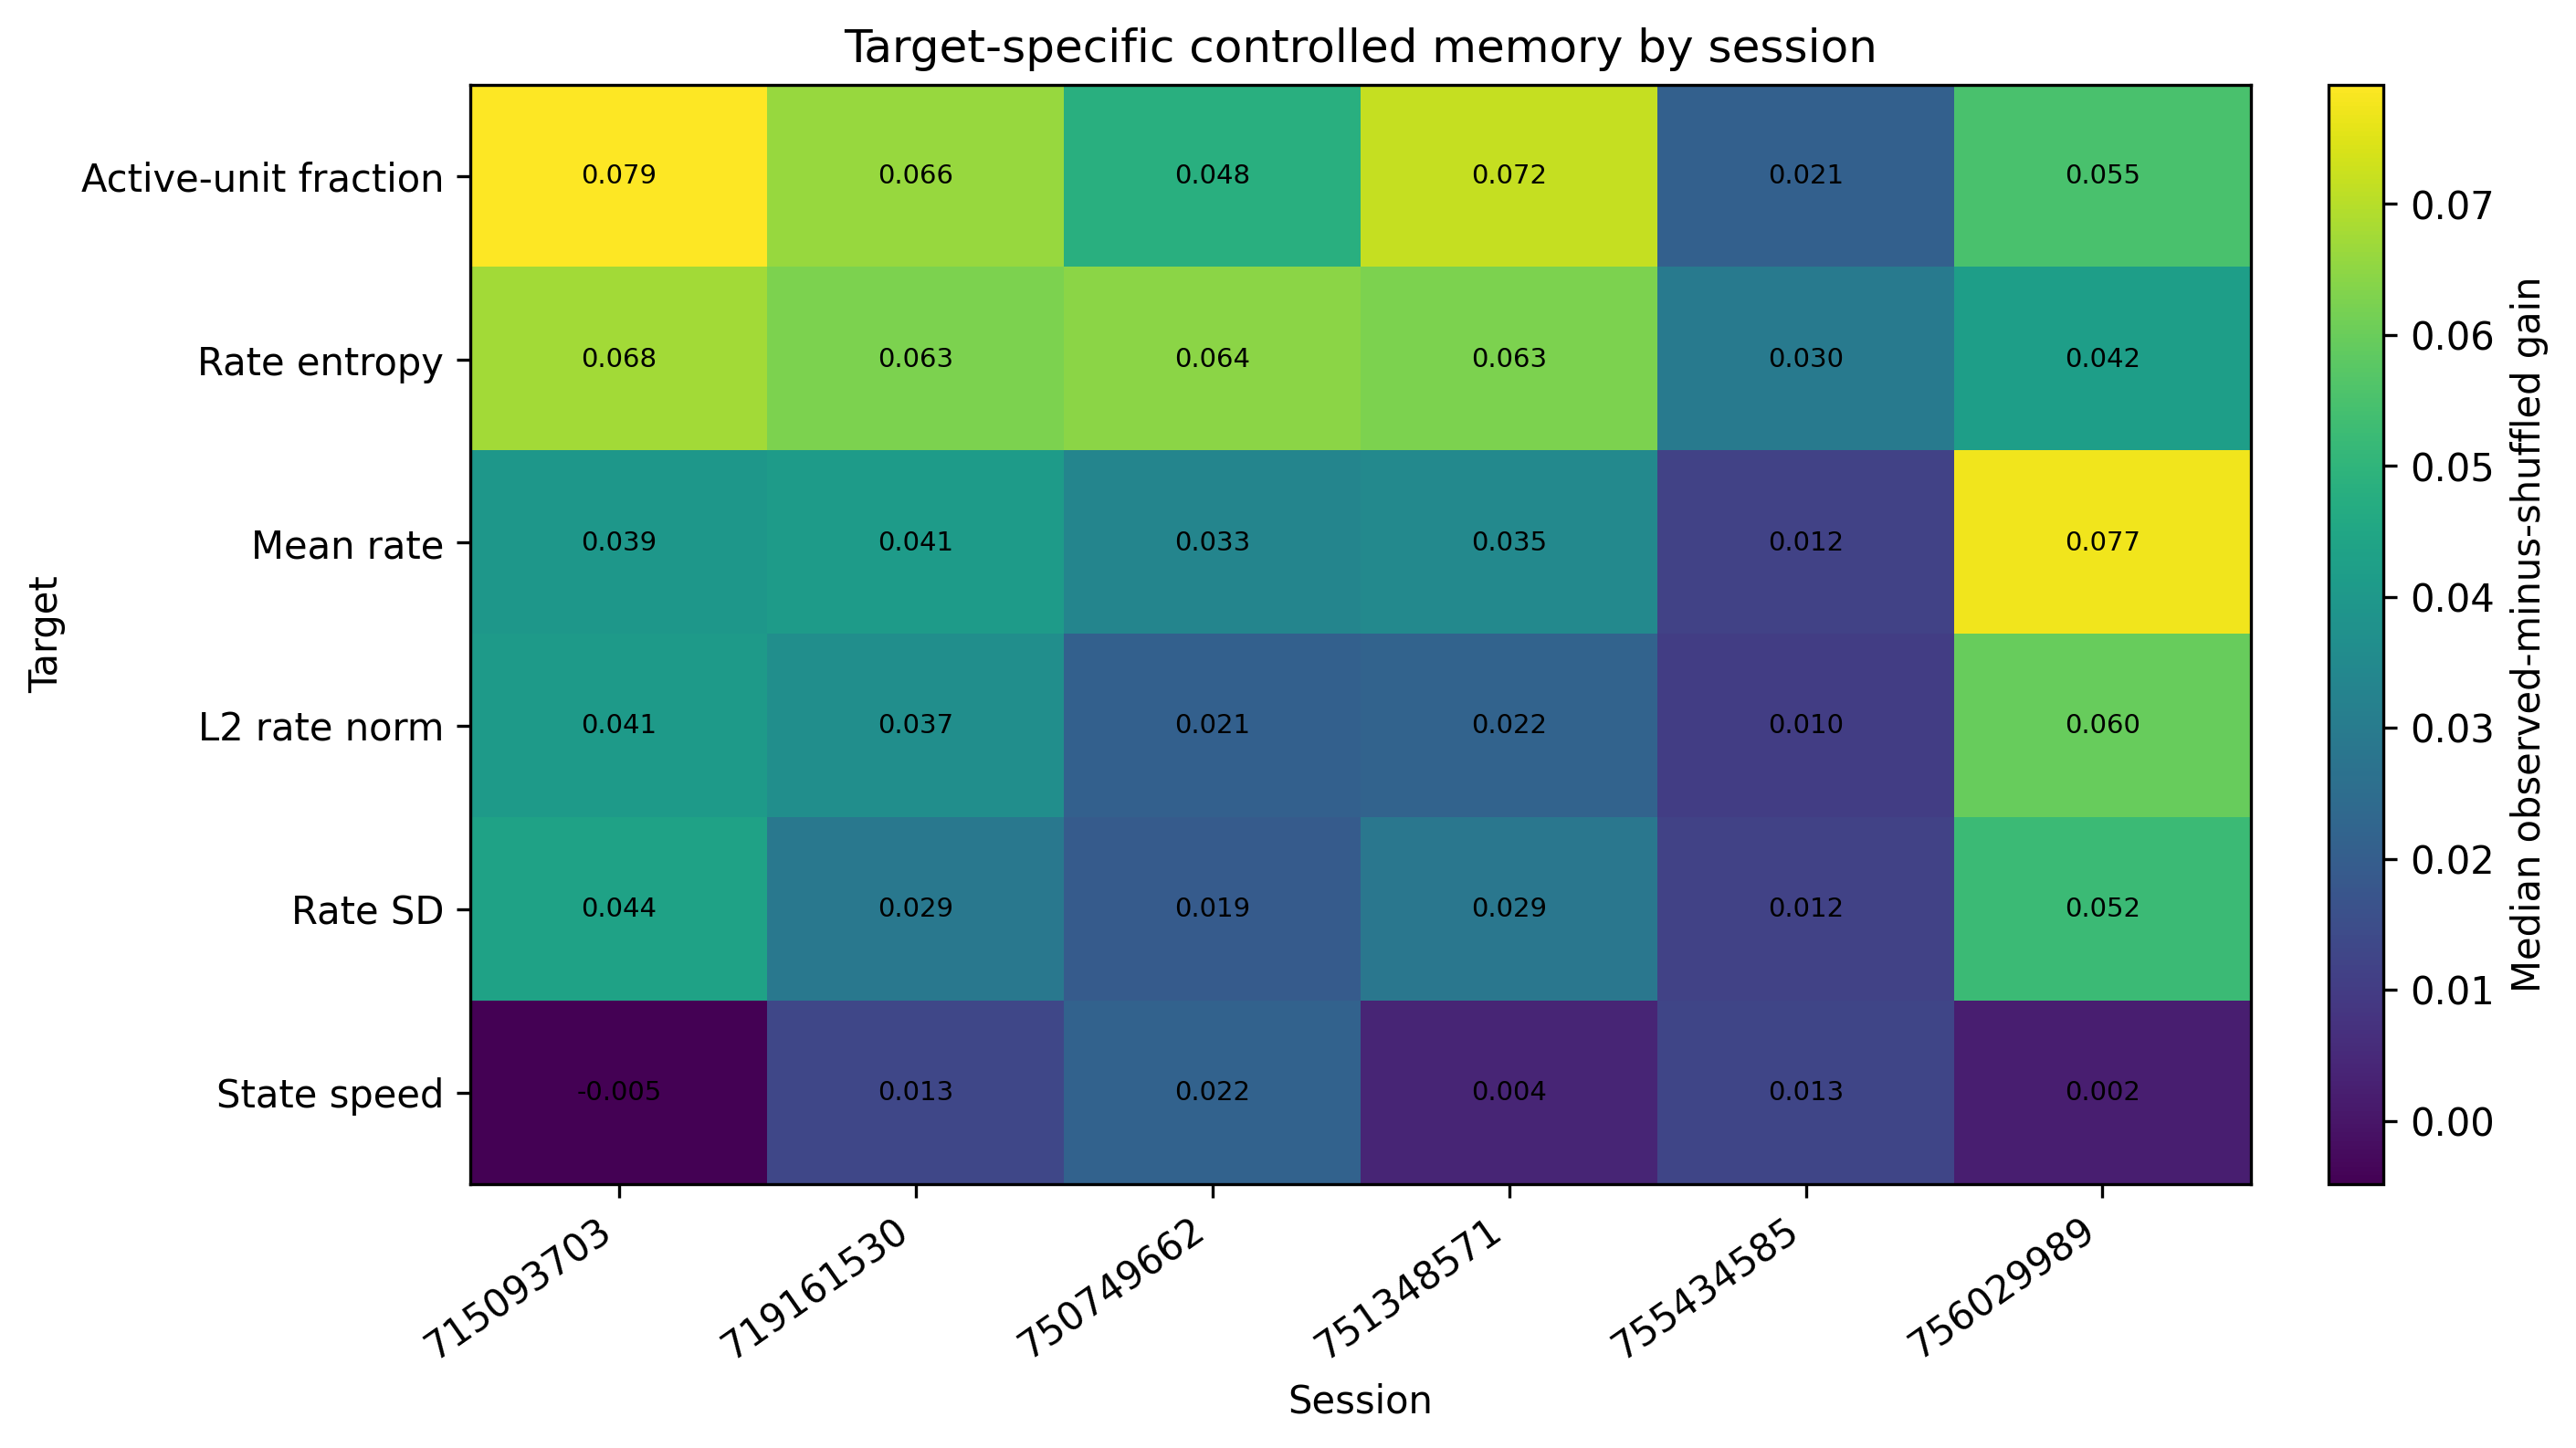
\includegraphics[width=0.9\linewidth]{results/figures/manuscript/allen_spontaneous_strict_v2/strict_v2_target_by_session_heatmap.png}
\caption{Target-specific controlled memory by session. Active-unit fraction and population-rate entropy are the strongest cross-session organizational targets, while population-state speed is weak across the cohort.}
\label{fig:strict-target-heatmap}
\end{figure}

\begin{figure}[t]
\centering
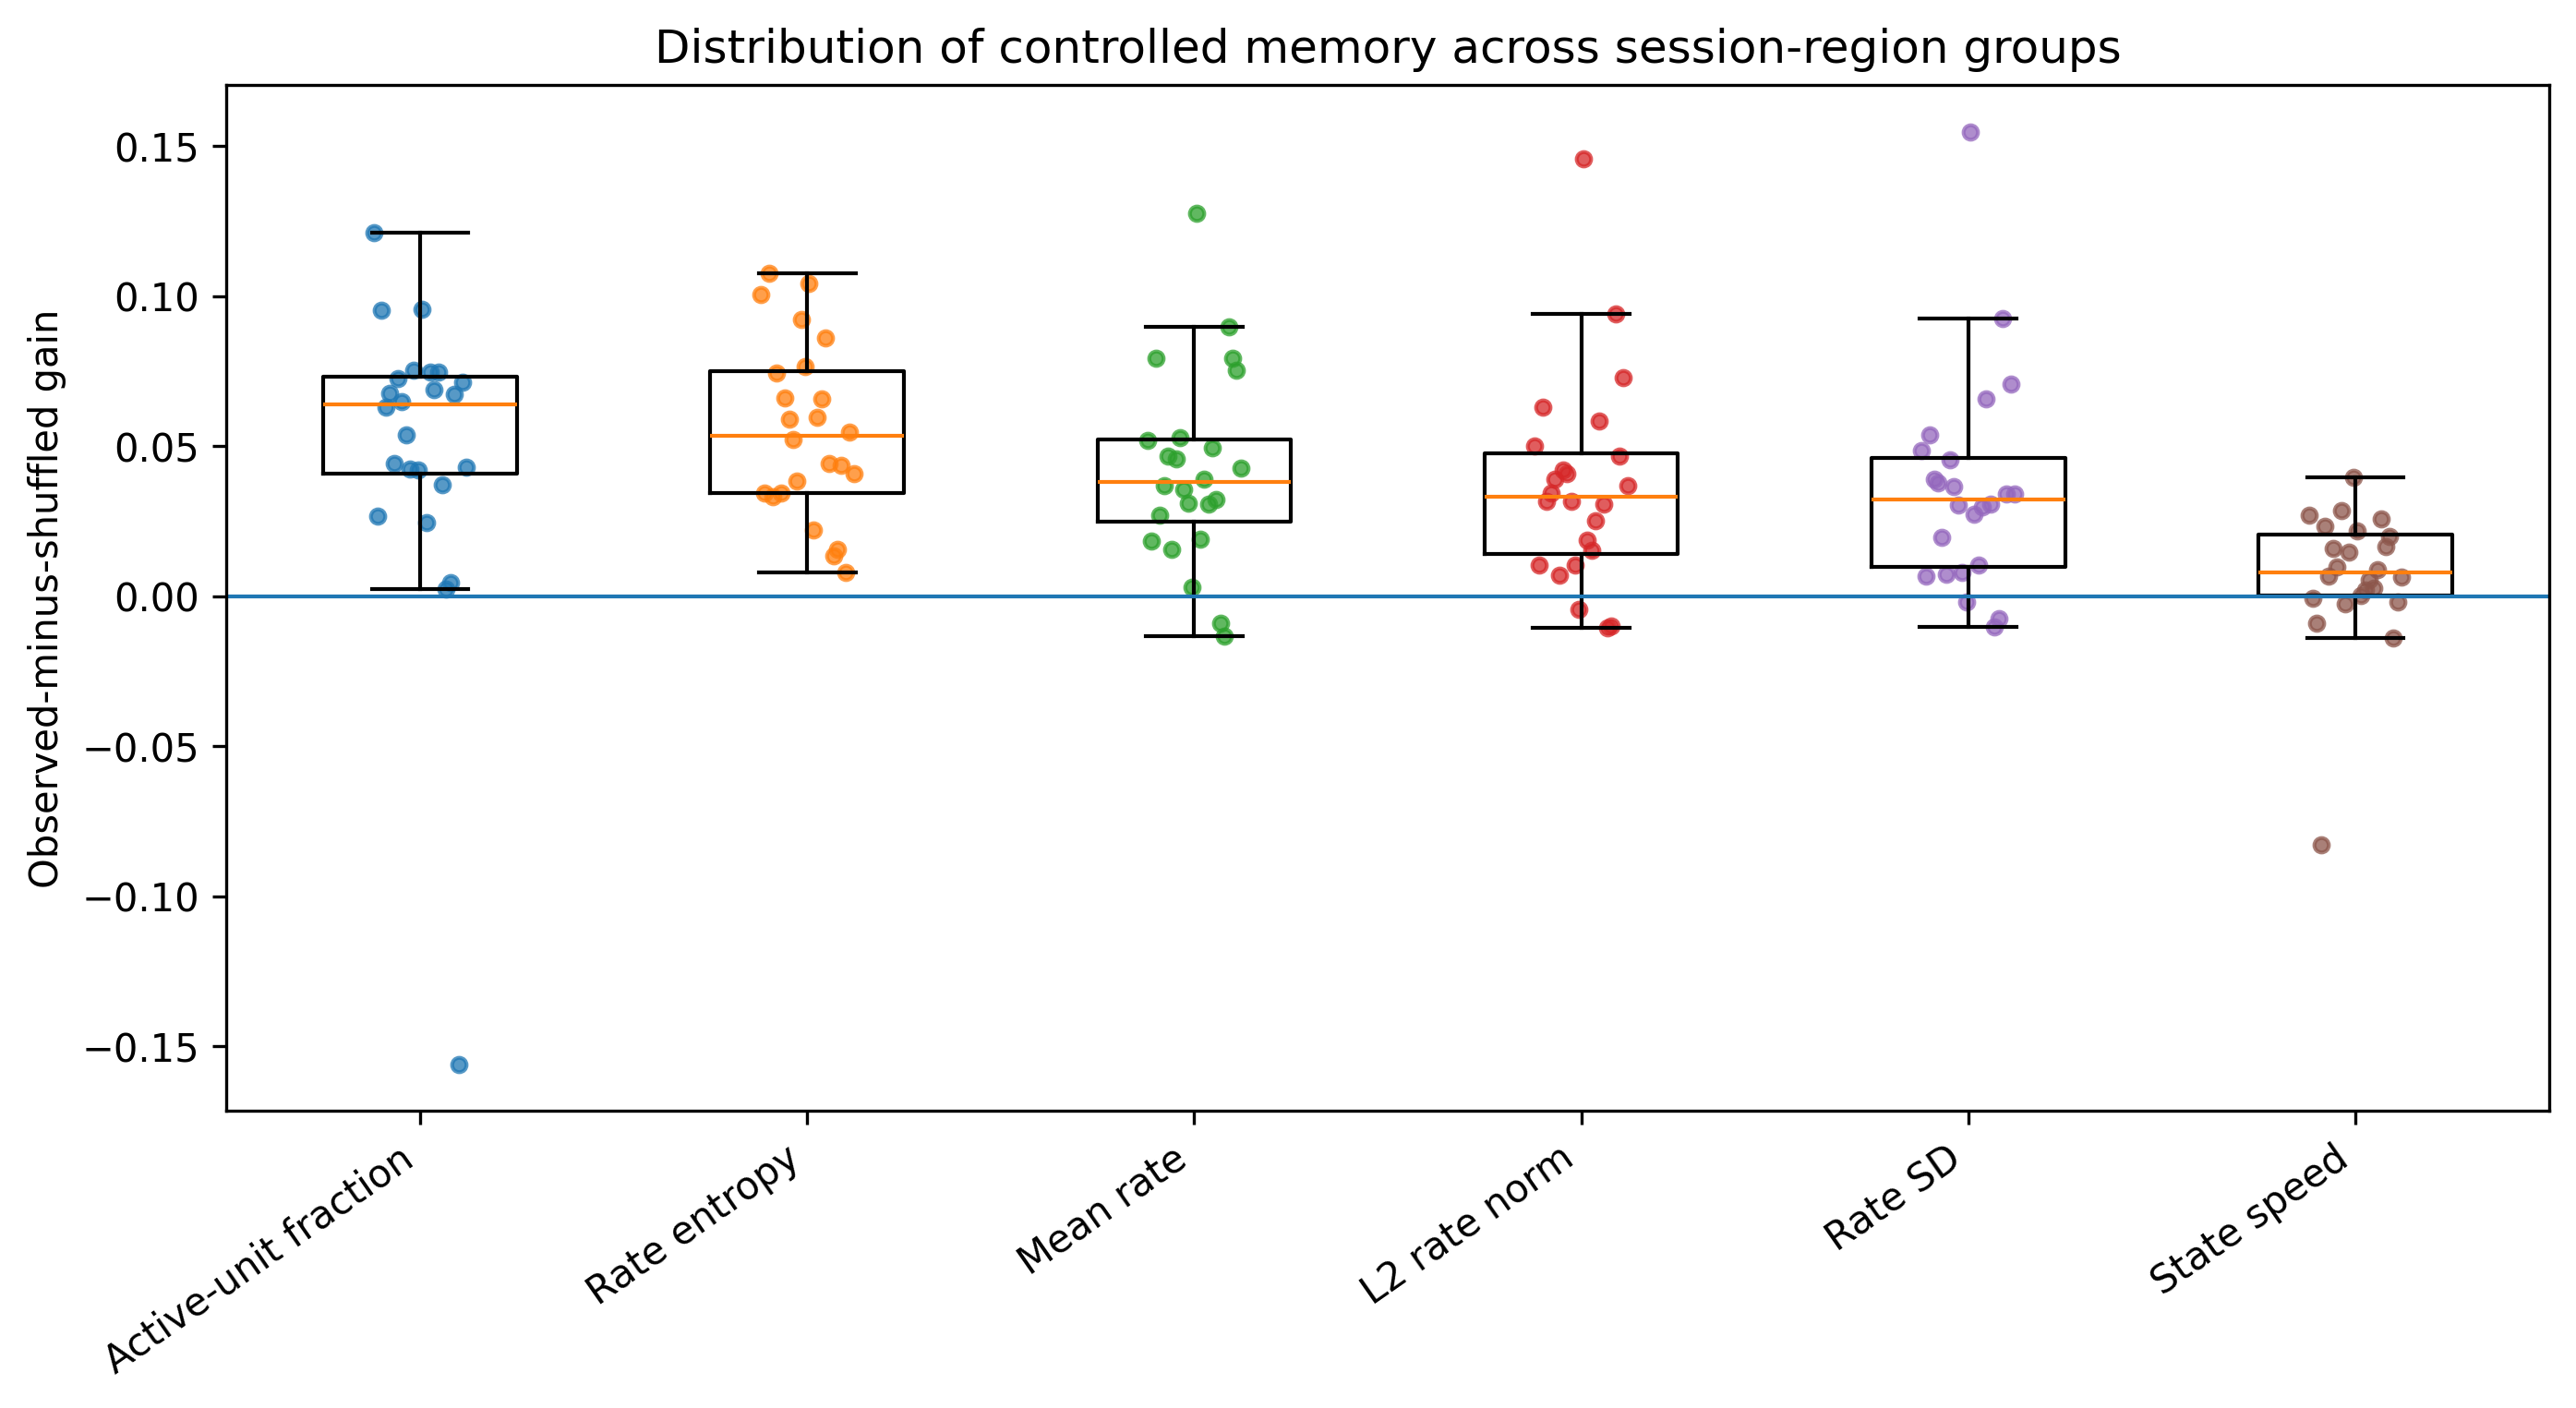
\includegraphics[width=0.86\linewidth]{results/figures/manuscript/allen_spontaneous_strict_v2/strict_v2_controlled_gain_distribution_by_target.png}
\caption{Distribution of controlled memory gains across session-region groups. The distributional view shows that recruitment and entropy remain favorable not only as cross-session medians but also across the underlying session-region groups.}
\label{fig:strict-gain-distribution}
\end{figure}

\subsection{Variance and autocorrelation residualization preserves the leading organizational targets}

A variance-scaling audit tested whether controlled memory gain tracked target variance, dispersion, or lag-1 autocorrelation. In the strict six-session cohort, active-unit fraction and population-rate entropy remained the top two targets after residualizing target variance, lag-1 autocorrelation, and row count. This strengthens the organizational-memory interpretation relative to the earlier three-session audit. The result is summarized in Table~\ref{tab:strict-variance} and Figure~\ref{fig:strict-variance}.

\begin{table}[t]
\centering
\caption{Variance and autocorrelation residualization in the strict six-session cohort.}
\label{tab:strict-variance}
\resizebox{\textwidth}{!}{%
\begin{tabular}{lrrrr}
\toprule
Target & Raw controlled gain & Raw rank & Residual gain & Residual rank \\
\midrule
active\_unit\_fraction & 0.064 & 1 & 0.006 & 1 \\
population\_rate\_entropy & 0.053 & 2 & 0.004 & 2 \\
population\_mean\_rate\_hz & 0.038 & 3 & -0.008 & 4 \\
population\_l2\_rate\_norm & 0.033 & 4 & 0.003 & 3 \\
population\_std\_rate\_hz & 0.032 & 5 & -0.009 & 5 \\
population\_state\_speed & 0.008 & 6 & -0.011 & 6 \\
\bottomrule
\end{tabular}%
}

\end{table}

\begin{figure}[t]
\centering
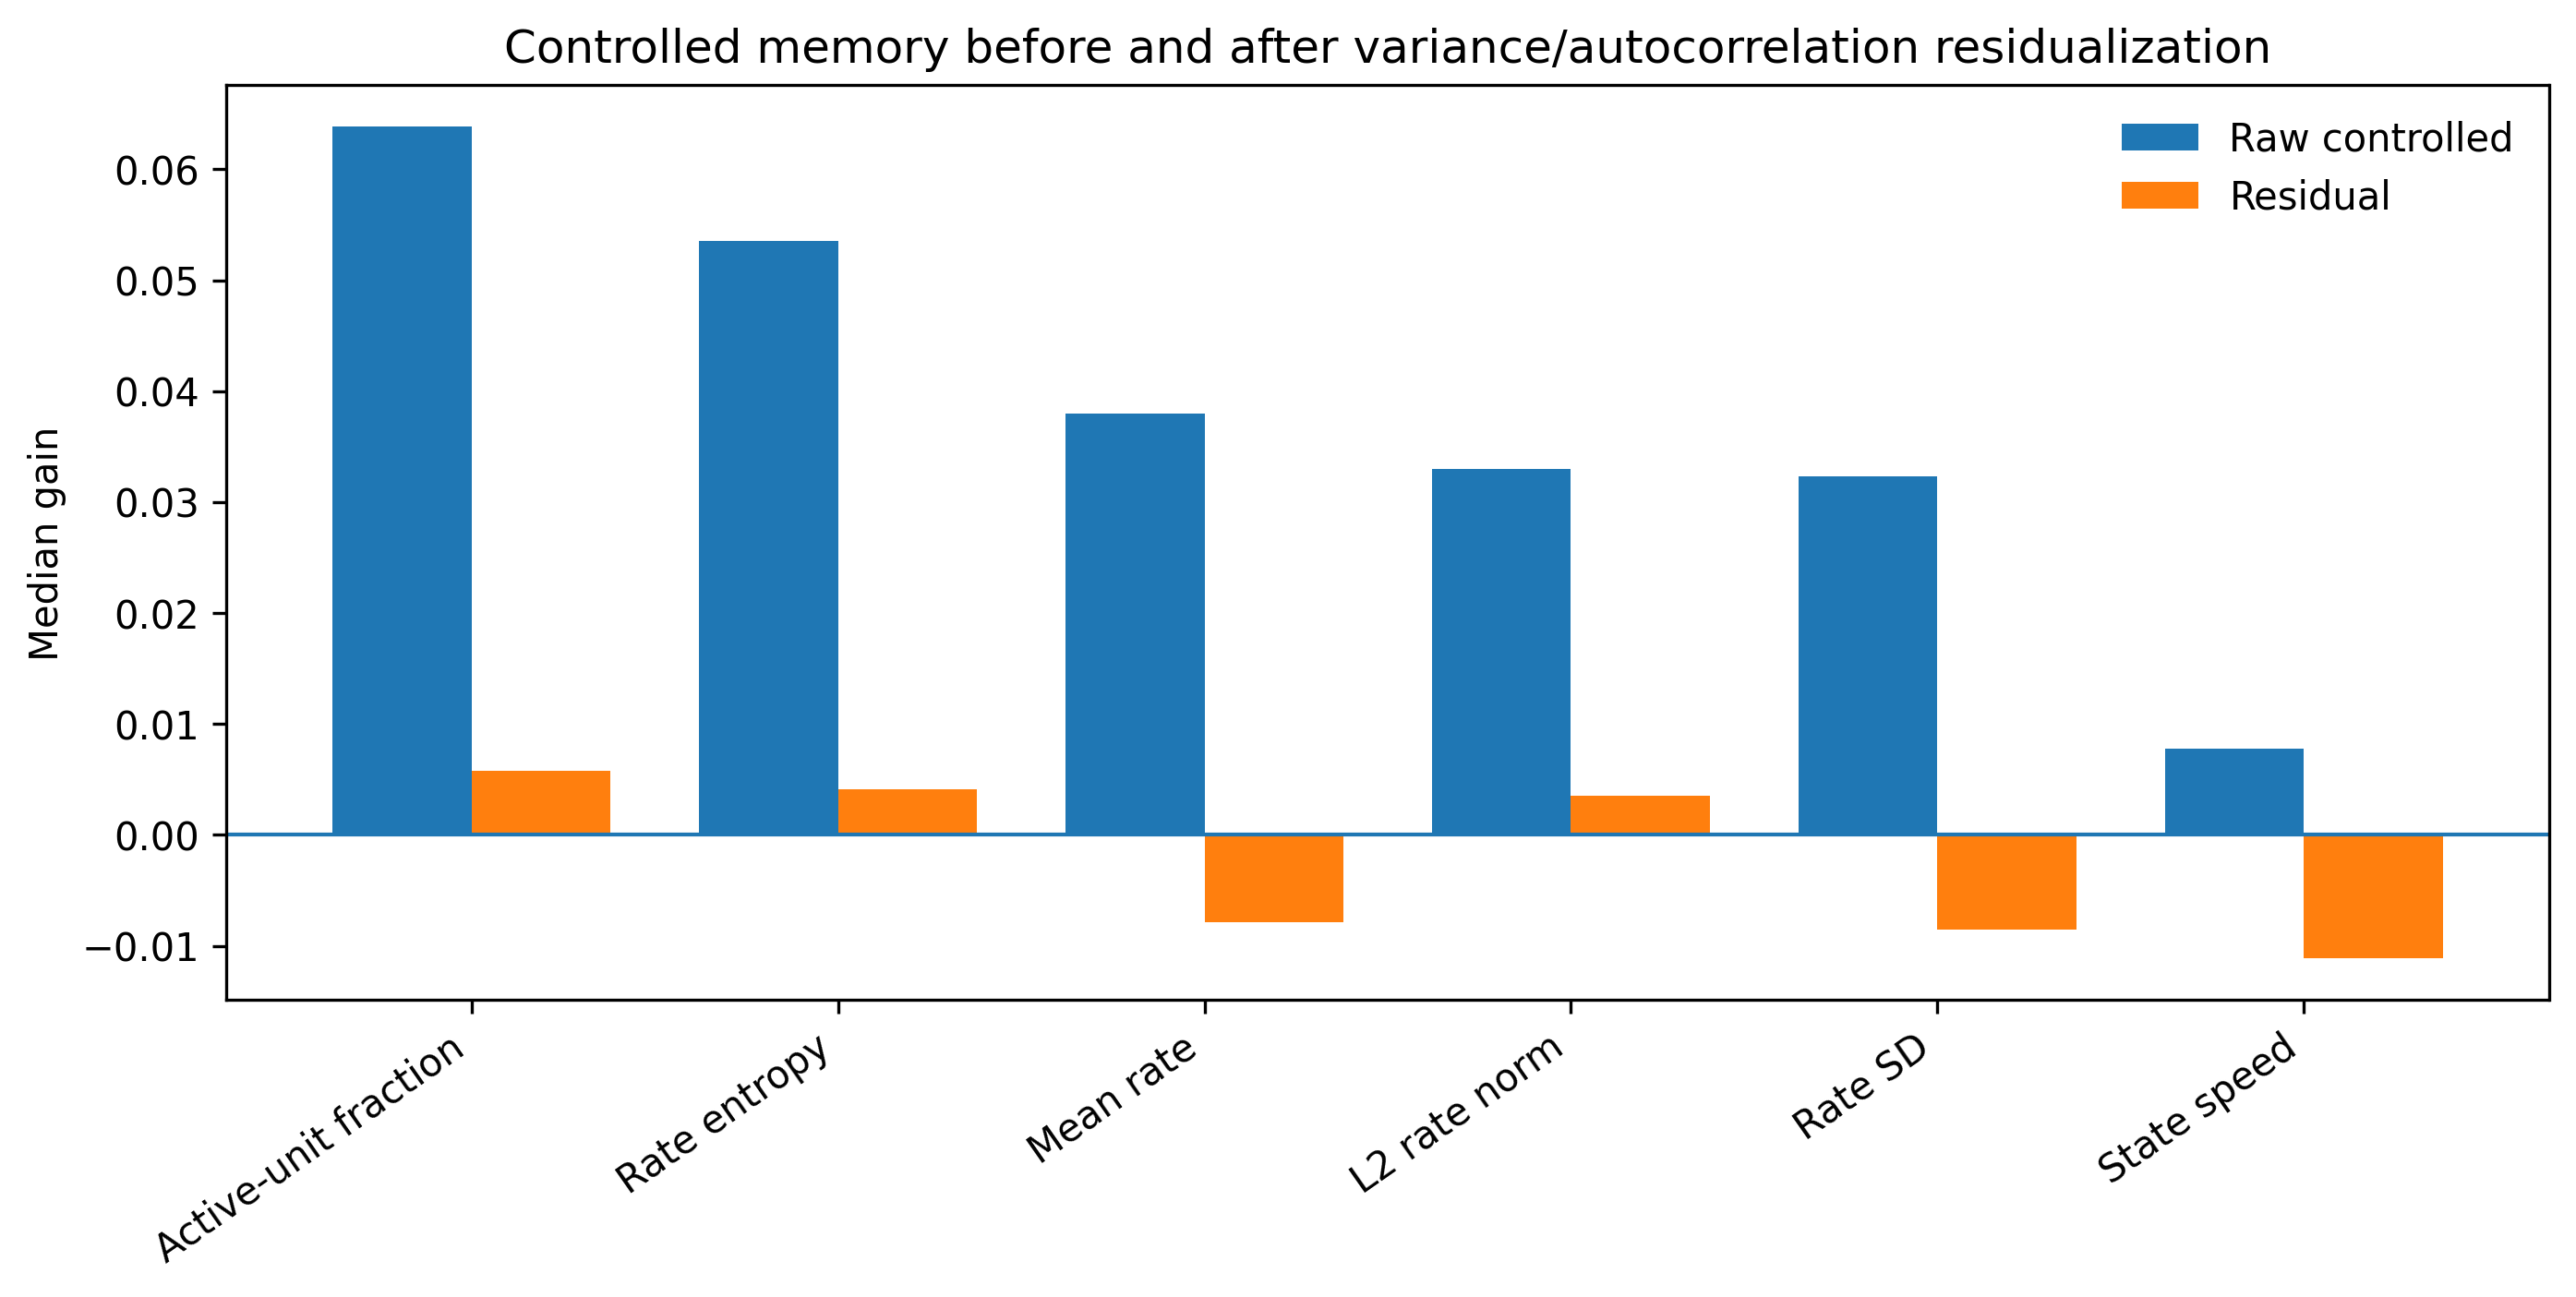
\includegraphics[width=0.88\linewidth]{results/figures/manuscript/allen_spontaneous_strict_v2/strict_v2_variance_residual_comparison.png}
\caption{Controlled memory before and after variance/autocorrelation residualization. Recruitment and entropy remain the leading targets after residualizing target variance, lag-1 autocorrelation, and row count.}
\label{fig:strict-variance}
\end{figure}

\subsection{Lag ablation supports a short distributed history window}

The six-session lag-ablation audit tested whether the memory contribution was exhausted by the nearest previous bin. It was not. Active-unit fraction and population-rate entropy remained positive across every tested lag set. Active-unit fraction increased from \StrictActiveLagOne{} under lag1 to \StrictActiveLagFour{} under lag1234. Population-rate entropy increased from \StrictEntropyLagOne{} under lag1 to \StrictEntropyLagFour{} under lag1234.

\begin{table}[t]
\centering
\caption{Strict six-session lag-ablation controlled gains. Values are median observed-minus-shuffled gains across sessions.}
\label{tab:strict-lag-ablation}
\resizebox{\textwidth}{!}{%
\begin{tabular}{lrrrrr}
\toprule
Target & lag1 & lag2 & lag12 & lag123 & lag1234 \\
\midrule
active\_unit\_fraction & 0.042 & 0.041 & 0.061 & 0.068 & 0.077 \\
population\_rate\_entropy & 0.038 & 0.046 & 0.063 & 0.075 & 0.081 \\
population\_mean\_rate\_hz & 0.025 & 0.029 & 0.037 & 0.044 & 0.046 \\
population\_state\_speed & 0.008 & 0.006 & 0.008 & 0.008 & 0.009 \\
\bottomrule
\end{tabular}%
}

\end{table}

\begin{figure}[t]
\centering
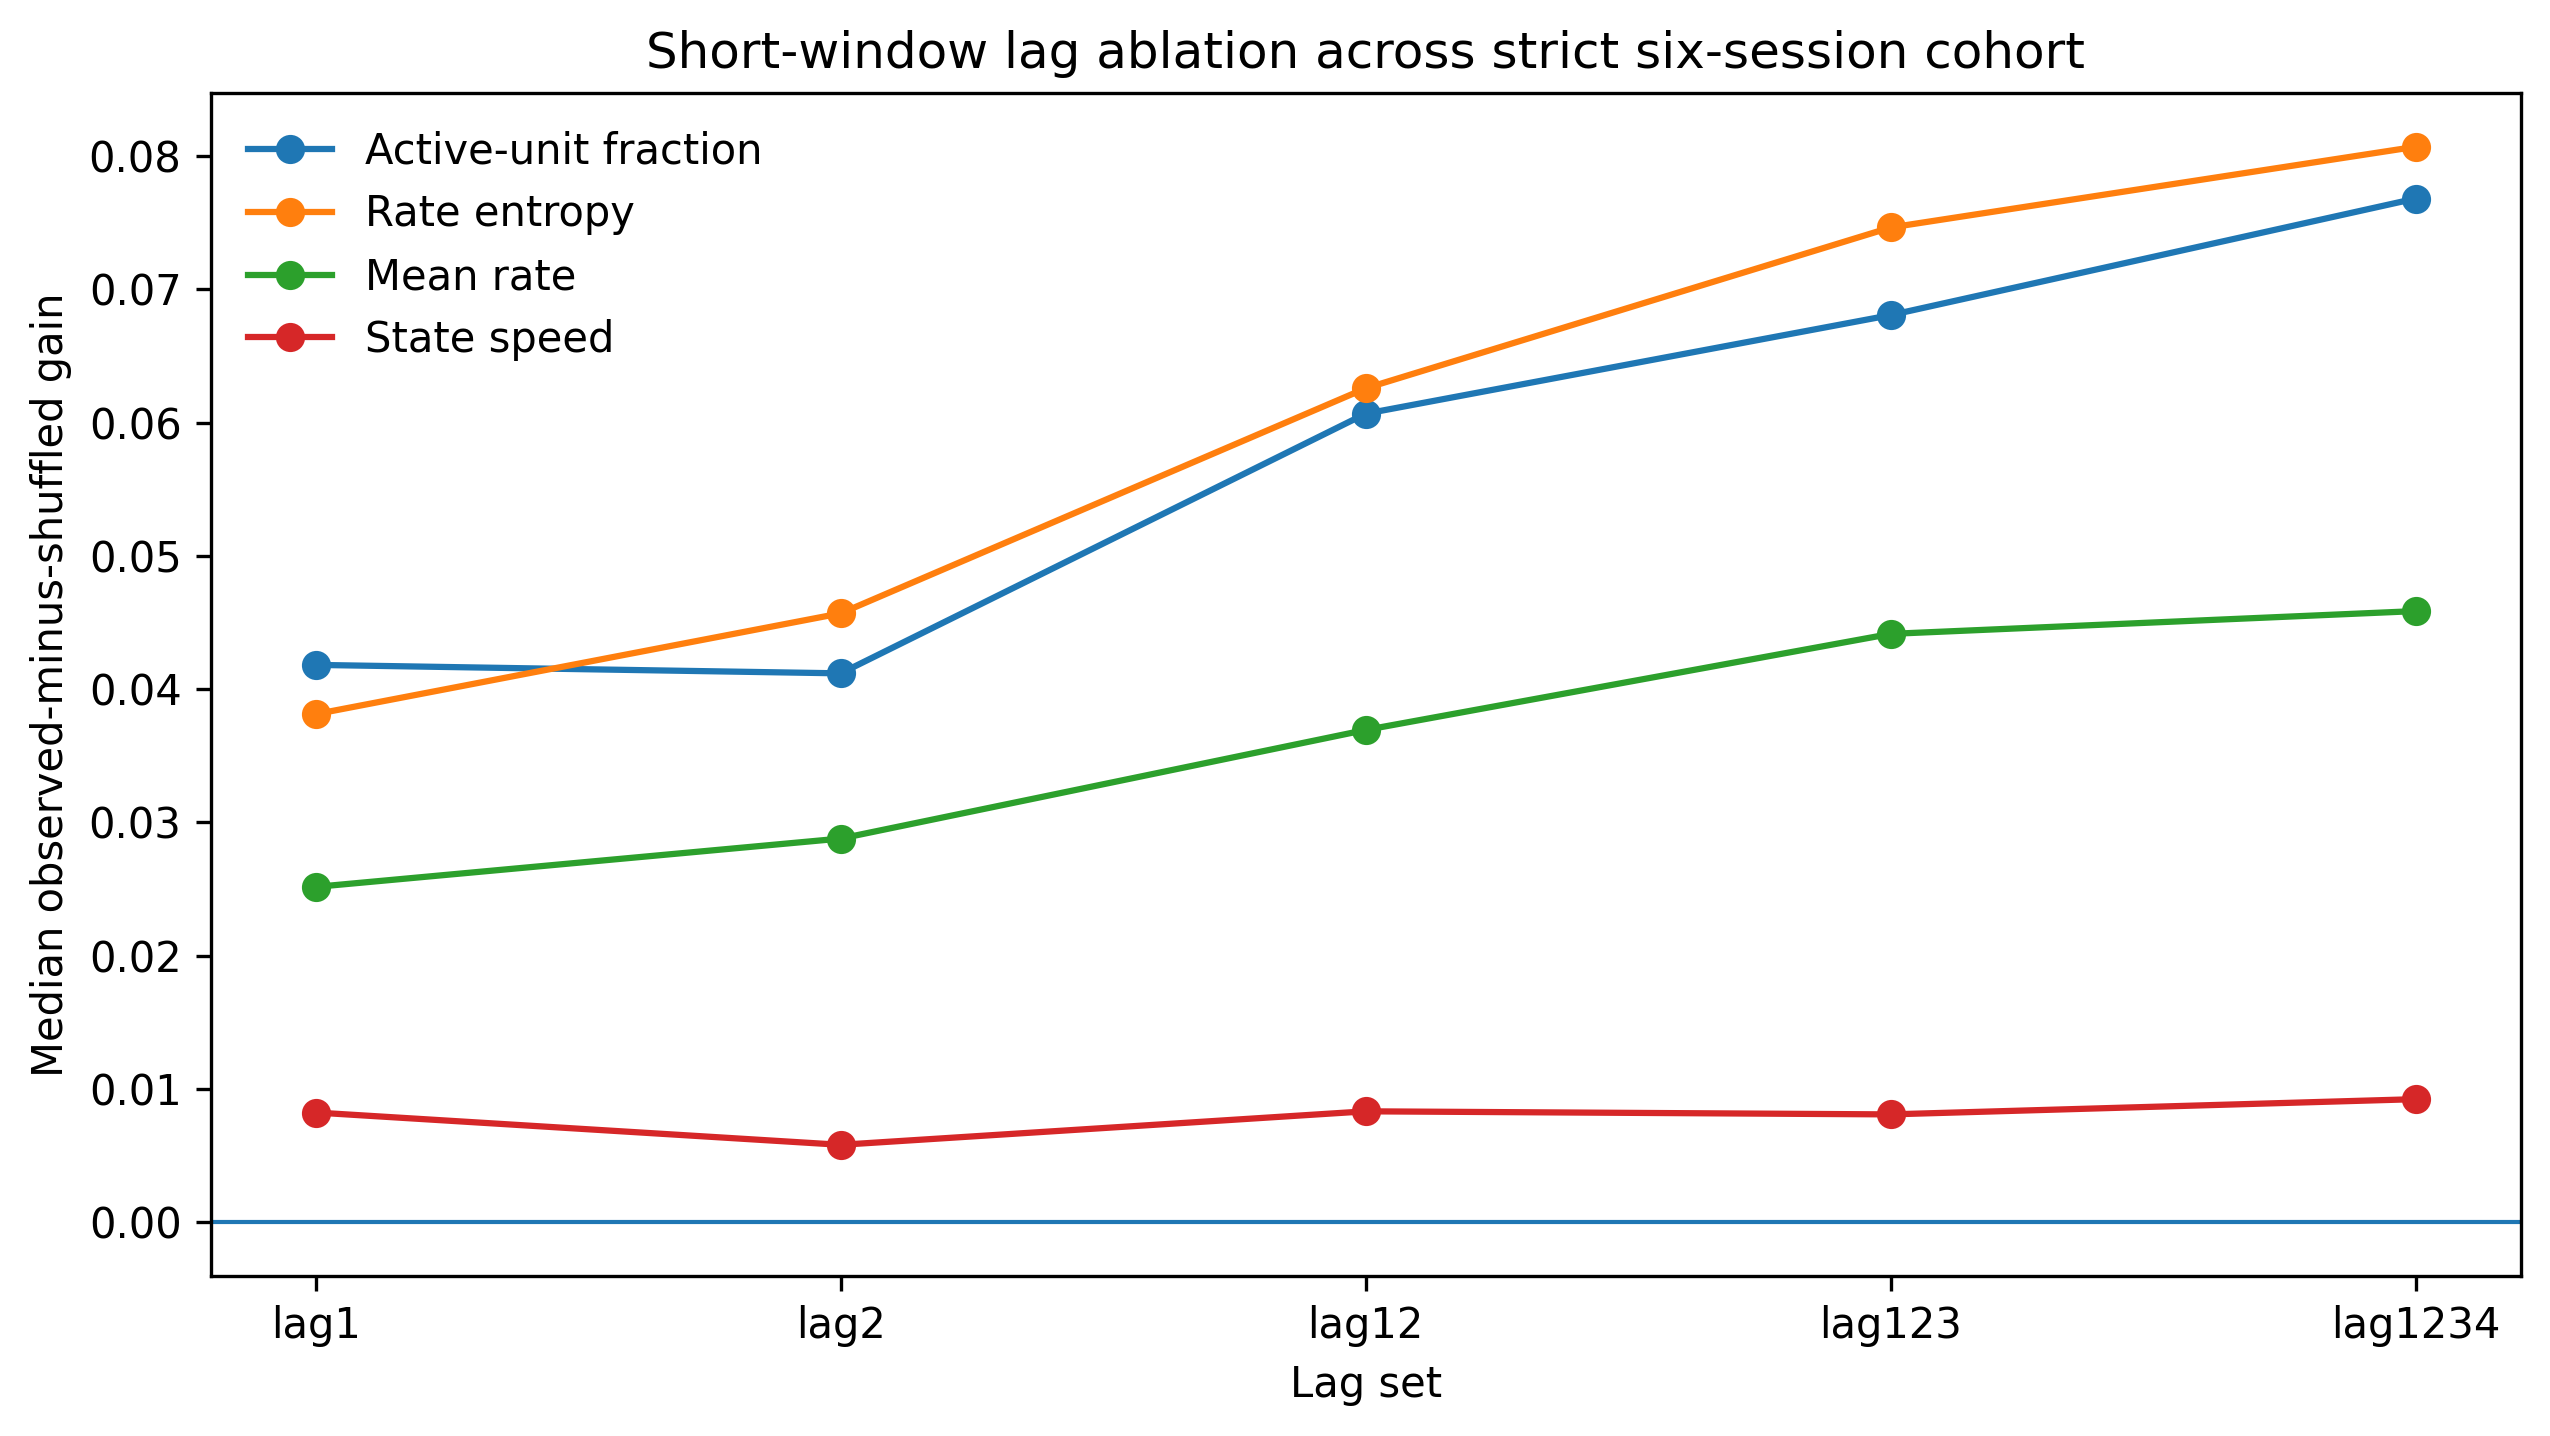
\includegraphics[width=0.88\linewidth]{results/figures/manuscript/allen_spontaneous_strict_v2/strict_v2_lag_ablation_curves.png}
\caption{Lag-ablation curves for the strict six-session cohort. Active-unit fraction and population-rate entropy remain positive across lag settings and increase across a short recent-history window.}
\label{fig:strict-lag-ablation}
\end{figure}

This supports an operational interpretation in which spontaneous population history is distributed across a short recent temporal window rather than reducible to the immediately preceding state. The result remains bounded: it establishes a predictive historical contribution under this model class, not a complete mechanistic theory of neural memory.

\subsection{Ripeness remains descriptive}

A descriptive spontaneous neural ripeness index was computed from rank-normalized \(\Phi_{\rm neural}\), stability \(S\), controlled mean-rate memory, active-unit memory, and entropy memory. This index is explicitly post hoc and descriptive. It includes memory gains as inputs and therefore cannot be used as independent evidence that high-ripeness states have high memory. Its value is organizational: it separates high-\(\Phi_{\rm neural}\) structural states from states carrying strong controlled organizational memory.

\begin{table}[t]
\centering
\caption{Region-level descriptive ripeness summary for the strict six-session cohort.}
\label{tab:strict-ripeness}
\resizebox{\textwidth}{!}{%
\begin{tabular}{lrrrrrrr}
\toprule
Region & $n$ & Median ripeness & Mean ripeness & Median $\Phi$ & Median active gain & Median entropy gain & Rank \\
\midrule
CA1 & 6 & 0.627 & 0.600 & -0.060 & 0.071 & 0.080 & 1 \\
VISl & 6 & 0.582 & 0.522 & -0.050 & 0.074 & 0.063 & 2 \\
LGd & 6 & 0.473 & 0.490 & 0.449 & 0.032 & 0.034 & 3 \\
VISp & 6 & 0.459 & 0.419 & 0.027 & 0.053 & 0.050 & 4 \\
\bottomrule
\end{tabular}%
}

\end{table}

\begin{figure}[t]
\centering
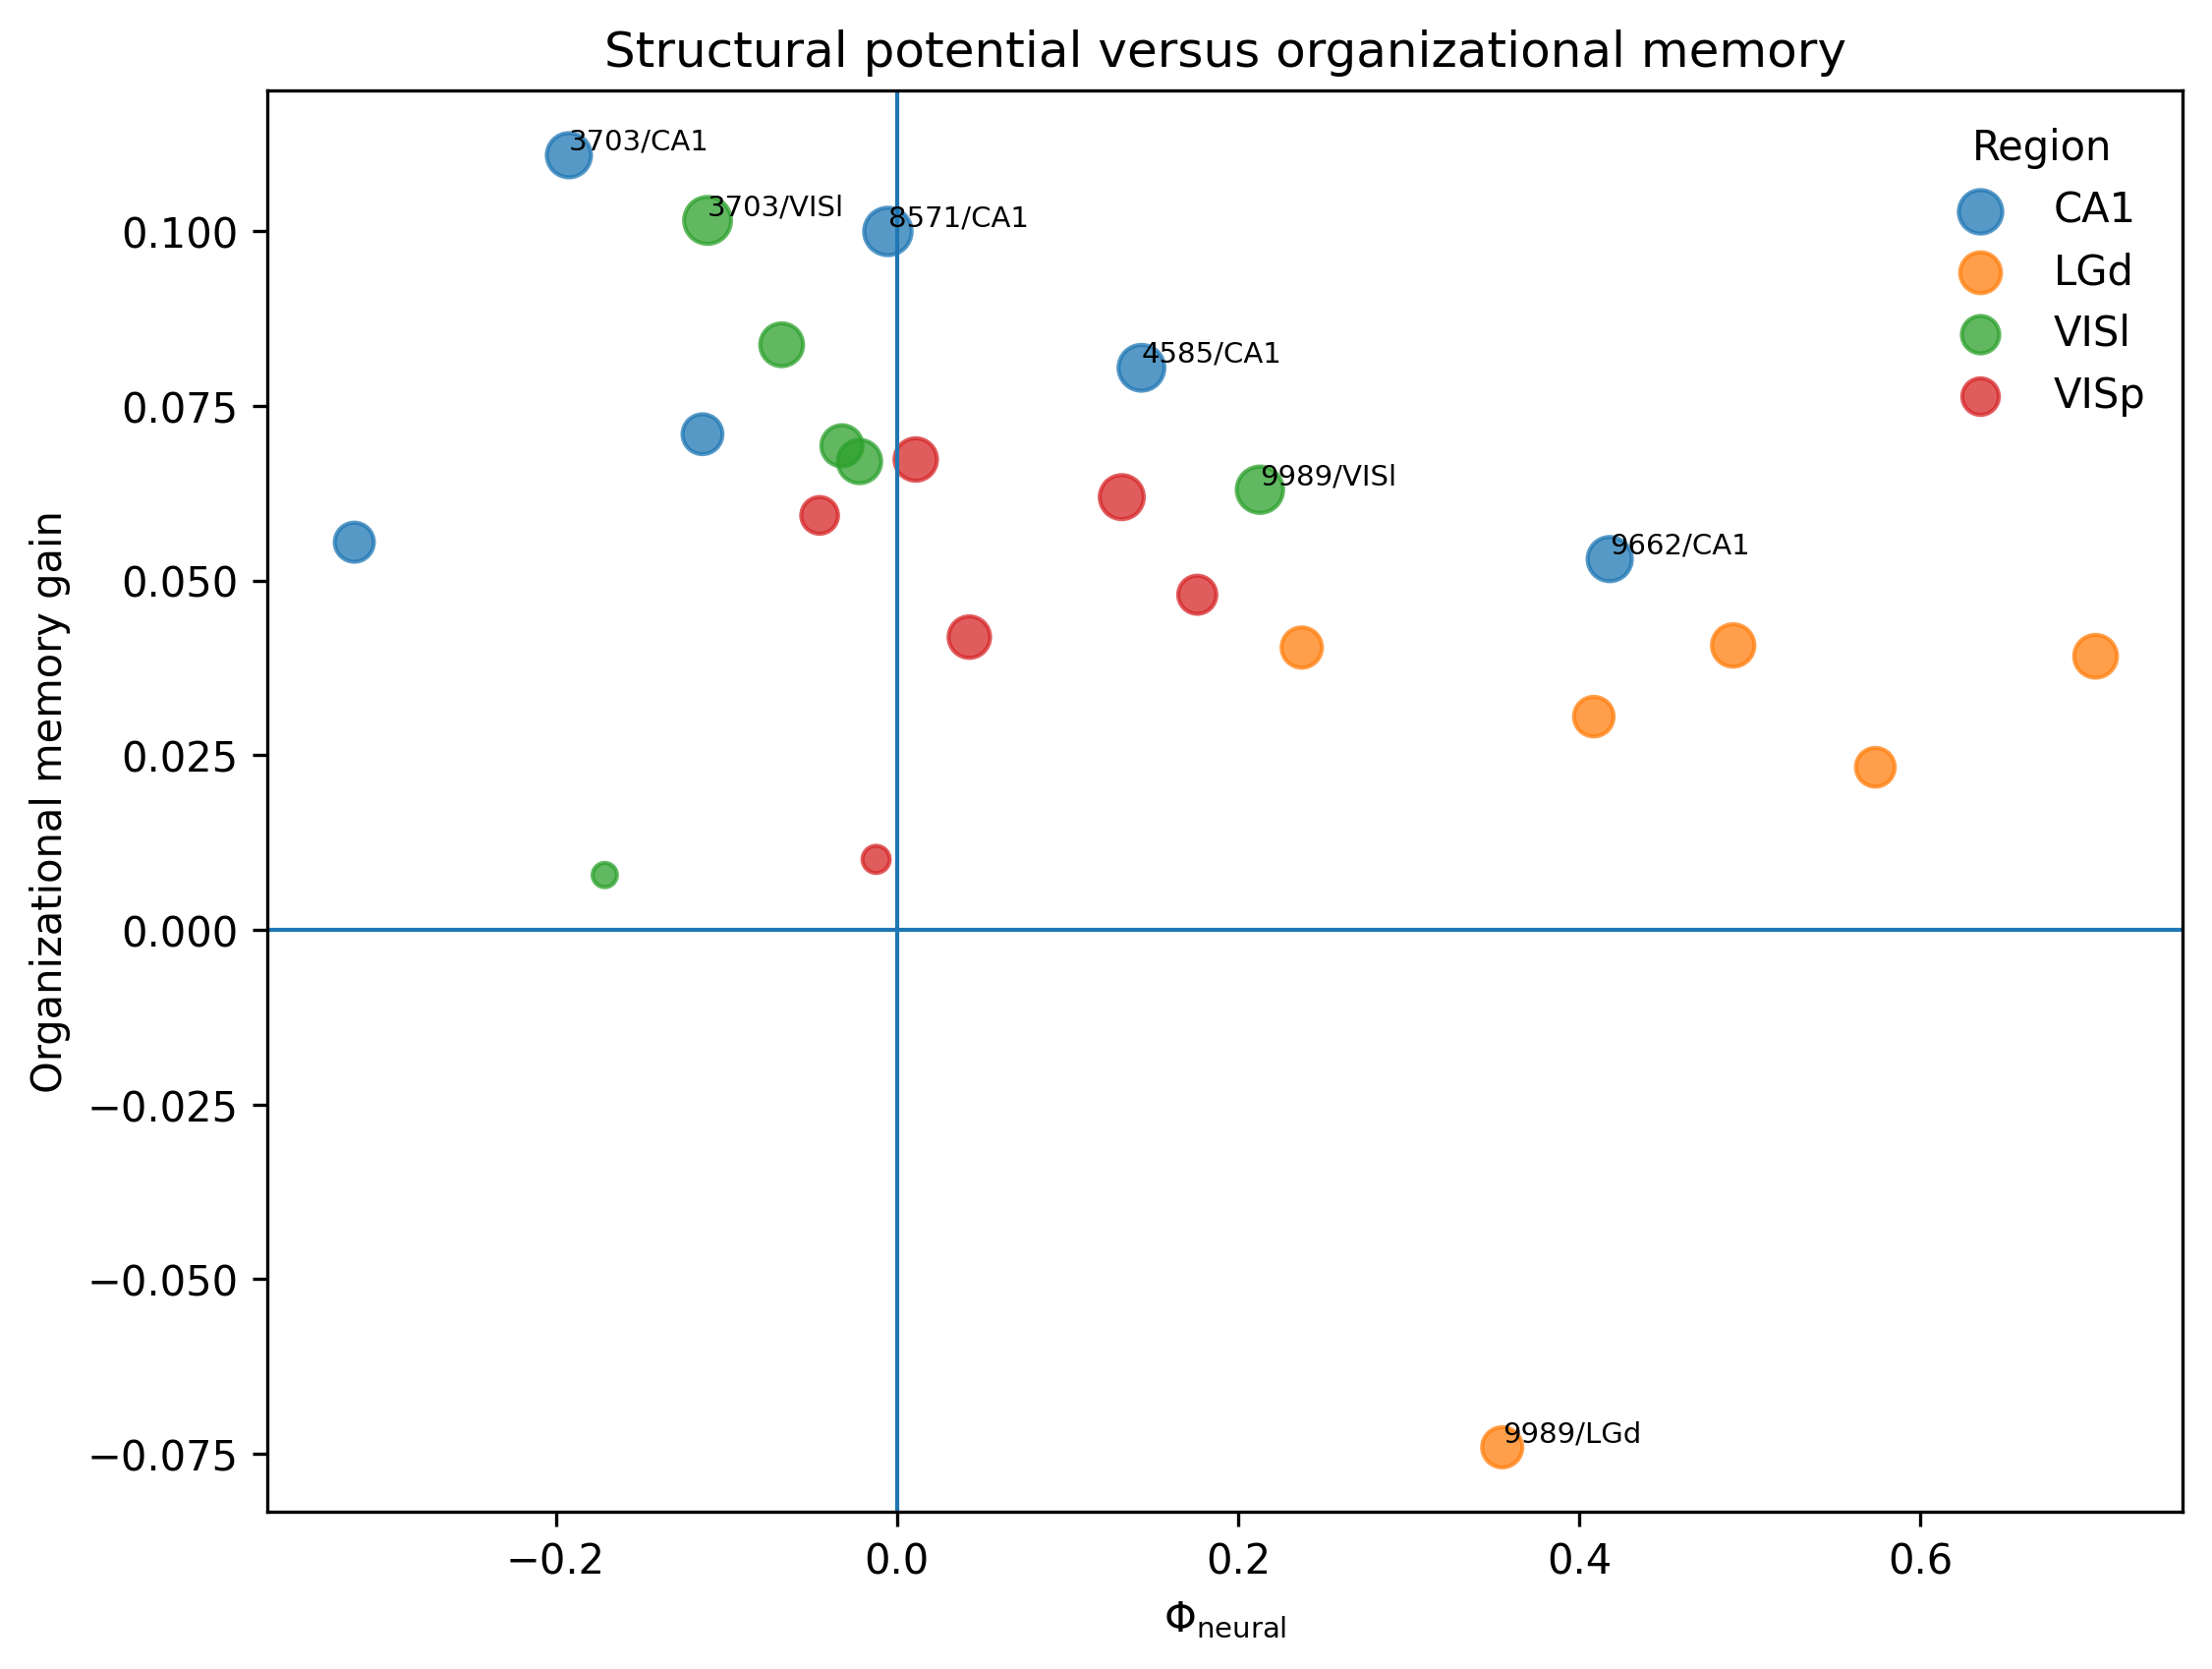
\includegraphics[width=0.82\linewidth]{results/figures/manuscript/allen_spontaneous_strict_v2/strict_v2_phi_memory_landscape_labeled.png}
\caption{Structural potential versus organizational memory in the strict six-session cohort. The plot separates high structural potential states from states carrying strong controlled organizational memory.}
\label{fig:strict-ripeness}
\end{figure}

\section{Discussion}

This analysis supports a bounded conclusion: spontaneous neural population activity contains controlled organizational memory. Across six strict fixed-scale Allen Brain Observatory Visual Coding Neuropixels sessions, active-unit fraction and population-rate entropy are the strongest cross-session controlled-memory targets. The effect survives shuffled-lag controls, variance/autocorrelation residualization, and lag-ablation testing.

The result should not be interpreted as universal mean-rate memory. Session 755434585 is a useful stress test because mean-rate memory is not uniformly positive across regions, yet entropy and active-unit fraction remain the leading organizational targets. The result should also not be interpreted as independent external replication. All sessions come from the same Allen Brain Observatory dataset, so the correct phrase is within-dataset cross-session generalization.

The target-level result is the conceptual center of the study. Active-unit fraction and population-rate entropy rank above mean firing rate in the strict cross-session synthesis. This suggests that retained history is most visible in how the population organizes itself: which units participate and how activity is distributed across the population. The lag-ablation audit reinforces this interpretation by showing that recruitment and entropy remain positive across all tested lag windows and increase as additional recent lags are included.

The HRSM coordinate audit also constrains the interpretation. Raw HRSM proxy axes are not assumed to be independent. Sequential residualization creates orthogonalized coordinates for state-space projection and downstream summaries. Therefore, near-zero post-residualization correlations verify the computation rather than proving independent biological axes. The raw-axis audit is included to make this distinction explicit.

Population-state speed remains the weakest target. This weak support is informative. State speed is a derivative-like quantity describing how rapidly the population state moves, whereas the present memory model uses recent population-position features. The result is therefore consistent with the interpretation that the retained-history signal is primarily structural and organizational, not kinetic. A stronger test of velocity or acceleration memory would require models that explicitly include velocity-like or acceleration-like predictors.

\section{Limitations}

The analysis remains within one public dataset. The six-session expansion strengthens within-dataset generalization but does not provide independent external replication. The HRSM coordinates are operational proxies and should not be treated as direct physiological variables. The residualized axes are useful for reduced state-space analysis, but their orthogonality is produced by the residualization procedure. The ripeness index is descriptive and partly circular because memory gains contribute to the score.

The shuffled-lag control is strong but not exhaustive. Other controls, including blockwise temporal shifts, circular shifts, region-label permutations, alternative model classes, and held-out unit resampling, should be tested in future work. The extraction scale is fixed at twenty units per region in the strict cohort; future sensitivity tests should evaluate 10-, 20-, and 30-unit extraction scales where data coverage allows.

\section{Conclusion}

A reduced HRSM state-space analysis of six strict fixed-scale Allen Brain Observatory Visual Coding Neuropixels spontaneous sessions reveals within-dataset cross-session generalization of controlled organizational memory. Active-unit fraction and population-rate entropy are the strongest cross-session targets. Both survive variance/autocorrelation residualization and remain positive across lag-ablation settings. Mean-rate memory is present but heterogeneous, and state-speed memory remains weak. The resulting claim is deliberately bounded: spontaneous neural population activity carries controlled organizational memory across a short recent history window.

\section*{Data availability}

No new animal data were generated. The analysis uses publicly available Allen Brain Observatory Visual Coding Neuropixels data \citep{AllenBrainObservatoryVisualCodingNeuropixels}. Derived summaries, figures, and scripts are stored in the accompanying repository and archived in the Zenodo reproducibility snapshot.

\section*{Code availability}

The analysis scripts are stored under \texttt{scripts/allen/} and \texttt{scripts/paper/}. The strict-v2 outputs used in this manuscript are stored under \texttt{results/cross\_session/allen\_spontaneous\_strict\_v2/}, \texttt{results/ablation/allen\_spontaneous\_strict\_v2/}, and \texttt{results/figures/}. The archived strict-v2 code and reproducibility snapshot is available on Zenodo at \href{https://doi.org/10.5281/zenodo.20724425}{10.5281/zenodo.20724425}.

\section*{Ethics statement}

This study reuses publicly released Allen Brain Observatory data. No new animal experiments were performed.

\section*{Competing interests}

The author declares no competing interests.

\section*{Author contributions}

S.A. designed the HRSM analysis framework, implemented the computational workflow, analyzed the Allen Neuropixels data, generated figures and robustness audits, and wrote the manuscript.

\section*{Acknowledgements}

The author acknowledges the Allen Institute for publicly releasing the Allen Brain Observatory Visual Coding Neuropixels dataset and associated documentation.

\bibliographystyle{plainnat}
\bibliography{paper/references}

\appendix

\section{Strict cohort and diagnostic session status}

The strict cohort contains six sessions with four regions and twenty units per region. Session 754312389 is excluded from the strict cohort and retained as a partial-coverage diagnostic because one region contributed fewer than twenty units.

\section{Machine-readable robustness flags}

The main machine-readable flags are stored in:
\[
\texttt{results/cross\_session/allen\_spontaneous\_strict\_v2/}
\]
and
\[
\texttt{results/ablation/allen\_spontaneous\_strict\_v2/}.
\]
The most important passing flags are that active-unit fraction and population-rate entropy are the top two raw and residualized cross-session targets, and that both remain positive across all lag-ablation settings. The most important failing flags are that universal all-region mean-rate memory and universal LGd dominance are not supported.

\section{Supplementary combined-session HRSM profile}

\begin{figure}[h]
\centering
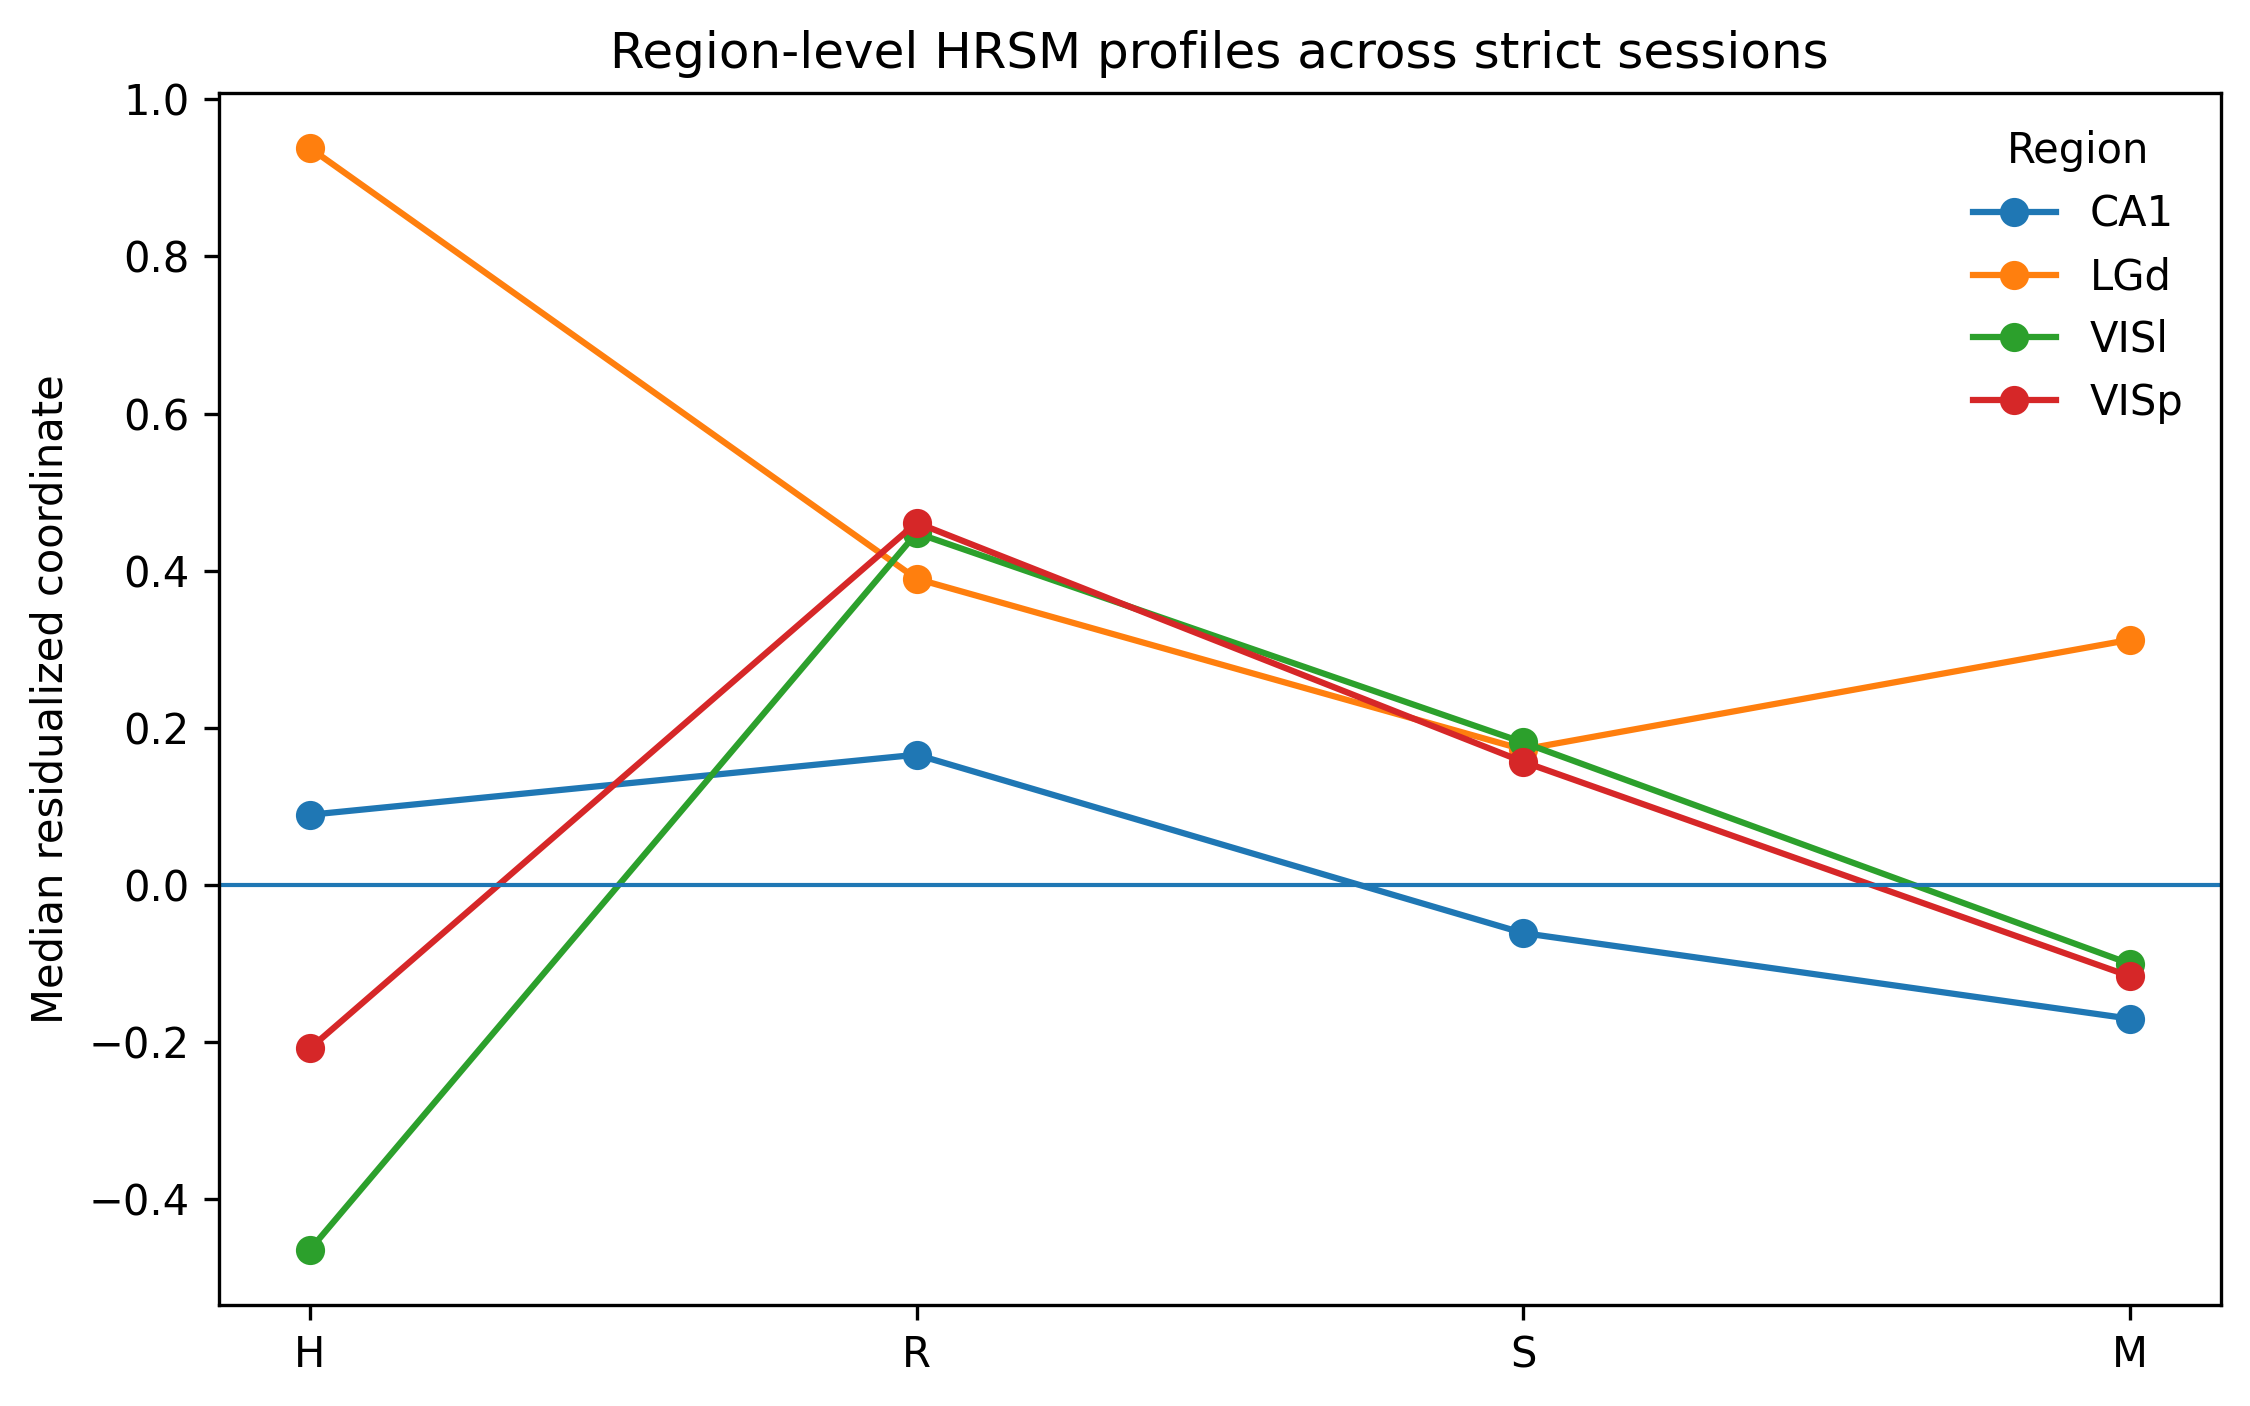
\includegraphics[width=0.9\linewidth]{results/figures/manuscript/allen_spontaneous_strict_v2/strict_v2_region_hrsm_profiles.png}
\caption{Median residualized \(H\), \(R\), \(S\), and \(M\) profiles by region across the six strict sessions. This figure is descriptive and should not be interpreted as direct physiological axis independence.}
\label{fig:region-hrsm-profiles}
\end{figure}

\end{document}
